\documentclass[journal,10pt,twocolumn]{IEEEtran}
\usepackage[utf8]{inputenc}
\usepackage[brazilian]{babel}
\usepackage{amsmath,amssymb,amsfonts}
\usepackage{graphicx}
\usepackage{booktabs}
\usepackage{cite}
\usepackage{hyperref}
\usepackage{geometry}
\geometry{top=19mm, bottom=19mm, left=15mm, right=15mm}

\title{\LARGE \bf Identificação de Sistemas SISO no Domínio da Frequência via Método N2CACGO: Da Fundamentação Analítica à Aplicação em Bancada Experimental de Motor CC}

\author{
    Renato Costa F\'{e}lix (Renato Felix), Jo\~{a}o Victor Tavares Pariz (Pariz),\\
    Pedro Augusto dos Santos Barbosa (Pedro Augusto), Wagner Scarpini Miranda (Scarpini)\\
    \textit{Faculdade de Engenharia El\'{e}trica, Instituto Militar de Engenharia (IME)}\\
    Pra\c{c}a General Tib\'{u}rcio, 80 -- Praia Vermelha, Rio de Janeiro -- RJ, Brasil\\
    \textit{Disciplina: Modelagem e An\'{a}lise de Sistemas Din\^{a}micos (MASD)}\\
    \textit{Docente: Prof. Dr. Marcelo de Ara\'{u}jo Oliveira}
}

\begin{document}

\maketitle

\begin{abstract}
A modelagem de sistemas dinâmicos baseada em identificação empírica no domínio da frequência constitui uma das ferramentas mais robustas da teoria de controle moderno, superando incertezas paramétricas e não-linearidades intrínsecas a modelos de primeiros princípios. Este trabalho implementa e valida computacionalmente a técnica \textbf{N2CACGO} (\textit{Norma 2 Convexo Analítico Conjunto Gerador Ótimo}), proposta na dissertação de mestrado de Bruno de Pinho Silveira no IME (2006). A técnica se destaca por formular o problema de estimação de funções de transferência SISO como uma otimização estritamente convexa em norma quadrática de erro de equação, fornecendo uma solução analítica global única via resolução de um Sistema de Equações Lineares (SEL) particionado, dispensando buscas heurísticas ou não-lineares. O método é submetido a rigorosa validação em três etapas: (i) reprodução dos resultados de referência de um sistema acadêmico de 7ª ordem com zeros (Silveira, 2006), alcançando exata concordância com as tabelas teóricas; (ii) integração temporal via simulação de sinal \textit{chirp} (0,1 a 15 Hz) com reconstrução espectral via Transformada Rápida de Fourier (FFT), recuperando a planta LTI com FIT de 96,5\%; e (iii) identificação prática da função de transferência de uma bancada experimental de motor elétrico CC ensaiada na disciplina de Sinais e Sistemas Lineares (SSL), demonstrando que um modelo de 1ª ordem com ganho $K \approx 10,08$ e constante de tempo mecânica $\tau_m \approx 0,21$~s atinge excelente precisão (RMSE de magnitude de 0,21~dB e FIT de 88,4\%), validado dinamicamente com respostas temporais a ondas quadrada e triangular.
\end{abstract}

\begin{IEEEkeywords}
Identificação de Sistemas, Resposta em Frequência, Método N2CACGO, Otimização Convexa, Motor de Corrente Contínua, FFT.
\end{IEEEkeywords}

\section{Introdução}
\IEEEPARstart{A}{obtenção} de modelos matemáticos fidedignos de sistemas dinâmicos é o pilar fundamental para o projeto de controladores, análise de estabilidade e previsão de desempenho operacional. Tradicionalmente, a modelagem por primeiros princípios (física ``caixa-branca'') deduz equações diferenciais baseando-se em leis constitutivas (e.g., leis de Newton, Kirchhoff ou termodinâmica). Todavia, na presença de geometrias complexas, saturação magnética, atrito não-linear e parâmetros térmicos variantes, os modelos dedutivos tornam-se de difícil calibração.

Nesse cenário, a \textbf{Identificação de Sistemas} (abordagem ``caixa-preta'' ou ``caixa-cinza'') constrói modelos matemáticos a partir de sinais de excitação aplicados na entrada e suas respectivas saídas mensuradas \cite{lathi2008,ogata2010}. Enquanto as abordagens no domínio do tempo (como ARX, ARMAX e PEM) são vulneráveis a ruídos de alta frequência e dependem fortemente de condições iniciais nulas, a abordagem no \textbf{domínio da frequência} oferece vantagens marcantes:
\begin{enumerate}
    \item Concentração natural da energia do sinal em frequências de interesse;
    \item Filtragem implícita de ruídos estocásticos fora da banda útil;
    \item Tratamento direto de atrasos de transporte e dinâmicas parasitárias.
\end{enumerate}

No Instituto Militar de Engenharia (IME), o desenvolvimento de metodologias no domínio da frequência culminou na formulação do método \textbf{N2CACGO} por Silveira \cite{silveira2006}, orientado na linha de pesquisa de controle e modelagem de sistemas dinâmicos. A grande inovação do N2CACGO reside na estruturação de um problema de otimização estritamente convexo, cuja solução ótima global é obtida de forma puramente \textbf{analítica}, superando limitações clássicas de convergência local inerentes a métodos de otimização não-linear baseados no algoritmo de Nelder-Mead (\texttt{fminsearch}) ou gradiente descendente.

O presente trabalho apresenta a implementação computacional completa do N2CACGO em ambiente MATLAB/Simulink e sua validação com exemplos acadêmicos, sinais simulados com FFT e ensaios experimentais reais de um motor de corrente contínua (CC).

\section{Fundamentação Teórica do Método N2CACGO}
\subsection{Estrutura do Modelo Estimado}
Considere um sistema linear e invariante no tempo (LTI), monovariável (SISO), cuja resposta em frequência empírica $G(j\omega_i)$ é conhecida para um conjunto discreto de $m$ frequências angulares:
\begin{equation}
    \Omega = \{\omega_1, \omega_2, \dots, \omega_m\}, \quad \omega_i \in \mathbb{R}^+
\end{equation}

Deseja-se ajustar uma Função de Transferência (FT) biprópria de ordem arbitrada $n$:
\begin{equation}
    G_e^n(s) = \frac{N(\alpha, s)}{D(\beta, s)} = \frac{\alpha_0 s^n + \alpha_1 s^{n-1} + \dots + \alpha_{n-1} s + \alpha_n}{s^n + \beta_1 s^{n-1} + \dots + \beta_{n-1} s + \beta_n}
    \label{eq:modelo_gen}
\end{equation}
onde os parâmetros a serem estimados são agrupados nos vetores:
\begin{equation}
    \alpha = [\alpha_0, \alpha_1, \dots, \alpha_n]^T \in \mathbb{R}^{n+1}
\end{equation}
\begin{equation}
    \beta = [\beta_1, \beta_2, \dots, \beta_n]^T \in \mathbb{R}^n
\end{equation}
\begin{equation}
    \theta = [\alpha^T, \; \beta^T]^T \in \mathbb{R}^{2n+1}
\end{equation}
com a imposição do coeficiente mônico $\beta_0 \triangleq 1$ no denominador para eliminar a redundância de escala.

\subsection{Função Custo e Convexidade}
A função custo direta $\| G(j\omega) - \frac{N(j\omega)}{D(j\omega)} \|_2^2$ resulta em um problema não-linear e não-convexo devido à presença dos parâmetros $\beta$ no denominador. Para viabilizar uma solução analítica global, o método N2CACGO adota o \textbf{erro de equação linearizado} ponderado em norma 2:
\begin{equation}
    J_S(\theta) = \| D(\beta, j\omega) G(j\omega) - N(\alpha, j\omega) \|_2^2
    \label{eq:custo_n2cacgo}
\end{equation}
que pode ser expandido discretamente sobre as $m$ frequências como:
\begin{equation}
    J_S(\theta) = \sum_{i=1}^m | D(\beta, j\omega_i) G(j\omega_i) - N(\alpha, j\omega_i) |^2
\end{equation}

A importância da convexidade reside na garantia matemática de que \textbf{todo mínimo local é necessariamente o mínimo global absoluto} \cite{marcelo2024}. Formalmente, uma função $f: X \to \mathbb{R}$ é dita convexa se, para quaisquer $x_1, x_2 \in X$ e qualquer $\lambda \in [0, 1]$:
\begin{equation}
    f(\lambda x_1 + (1-\lambda) x_2) \le \lambda f(x_1) + (1-\lambda) f(x_2)
    \label{eq:def_convexa}
\end{equation}
Em termos de cálculo diferencial multivariado, isso equivale a exigir que a matriz Hessiana seja semidefinida positiva ($\nabla^2 f(\theta) \ge 0$) em todo o domínio. No caso da Eq. (\ref{eq:custo_n2cacgo}), o resíduo $e(\theta, j\omega_i) = D(\beta, j\omega_i) G(j\omega_i) - N(\alpha, j\omega_i)$ é \textbf{estritamente linear} nos parâmetros $\theta = [\alpha^T, \beta^T]^T$. Consequentemente, o Hessiano $\nabla^2 J_S(\theta) = 2 \text{Re}\{A^H A\}$ é constante e estritamente positivo definido.

Esse resultado supera de forma definitiva as limitações de abordagens clássicas, como a Técnica de Imposição de Polos de Valle \cite{valle2005}, a qual não é convexa, não permite o cálculo analítico fechado de todos os parâmetros e fica sujeita a convergências espúrias em mínimos locais. No N2CACGO, a otimalidade global é atingida analiticamente anulando-se o gradiente:
\begin{equation}
    \nabla_\theta J_S(\theta) = \mathbf{0}_{(2n+1) \times 1} \implies \begin{cases}
        \frac{\partial J_S}{\partial \alpha_k} = 0, & k = 0, \dots, n \\
        \frac{\partial J_S}{\partial \beta_l} = 0, & l = 1, \dots, n
    \end{cases}
\end{equation}

\subsection{Dedução Matricial do Sistema Linear}
Definindo o vetor de potências de frequência $R_k(j\omega_i) \triangleq (j\omega_i)^k$ e $\Gamma(j\omega_i) \triangleq G(j\omega_i) G^*(j\omega_i) = |G(j\omega_i)|^2$, a diferenciação resulta em:
\begin{equation}
    \sum_{i=1}^m \text{Re} \left[ R_{n-k} N^*(\alpha) - R_{n-k} G^* D^*(\beta) \right] = 0
\end{equation}
\begin{equation}
    \sum_{i=1}^m \text{Re} \left[ R_{n-l} \Gamma D^*(\beta) - R_{n-l} G N^*(\alpha) \right] = 0
\end{equation}

Agrupando os termos lineares em $\alpha$ e $\beta$, e isolando os termos independentes decorrentes de $\beta_0 = 1$, obtém-se o Sistema de Equações Lineares (SEL):
\begin{equation}
    Q \theta = Y \iff \begin{bmatrix} Q_1 & -Q_2 \\ Q_3 & -Q_4 \end{bmatrix} \begin{bmatrix} \alpha \\ \beta \end{bmatrix} = \begin{bmatrix} Y_1 \\ Y_2 \end{bmatrix}
    \label{eq:sel_n2cacgo}
\end{equation}

Para implementação computacional vetorizada de alta eficiência, define-se a matriz de base polinomial $R \in \mathbb{C}^{(n+1) \times m}$:
\begin{equation}
    R = \begin{bmatrix}
        (j\omega_1)^n & (j\omega_2)^n & \dots & (j\omega_m)^n \\
        (j\omega_1)^{n-1} & (j\omega_2)^{n-1} & \dots & (j\omega_m)^{n-1} \\
        \vdots & \vdots & \ddots & \vdots \\
        1 & 1 & \dots & 1
    \end{bmatrix}
\end{equation}
e as matrizes diagonais dos dados espectrais $S = \text{diag}(G(j\omega_i))$ e $S^* = \text{diag}(G^*(j\omega_i))$.

Os blocos matriciais da Eq. (\ref{eq:sel_n2cacgo}) são calculados analiticamente por produtos matriciais diretos:
\begin{align}
    Q_1 &= \text{Re} \{ R \cdot R^H \} \quad \in \mathbb{R}^{(n+1) \times (n+1)} \\
    Q_2 &= \text{Re} \{ R \cdot S^* \cdot R^H(:, 2:n+1) \} \quad \in \mathbb{R}^{(n+1) \times n} \\
    Q_3 &= \text{Re} \{ R(2:n+1, :) \cdot S \cdot R^H \} \quad \in \mathbb{R}^{n \times (n+1)} \\
    Q_4 &= \text{Re} \{ R(2:n+1, :) \cdot S \cdot S^* \cdot R^H(:, 2:n+1) \} \quad \in \mathbb{R}^{n \times n}
\end{align}
e os vetores de excitação independente são dados por:
\begin{align}
    Y_1 &= \text{Re} \{ R \cdot S^* \cdot R^H(:, 1) \} \quad \in \mathbb{R}^{n+1} \\
    Y_2 &= \text{Re} \{ R(2:n+1, :) \cdot S \cdot S^* \cdot R^H(:, 1) \} \quad \in \mathbb{R}^n
\end{align}
onde $(\cdot)^H$ denota o operador transposto conjugado (Hermitiano). A solução é obtida imediatamente por $\theta = Q^{-1} Y$.


\begin{figure}[htbp]
\centering
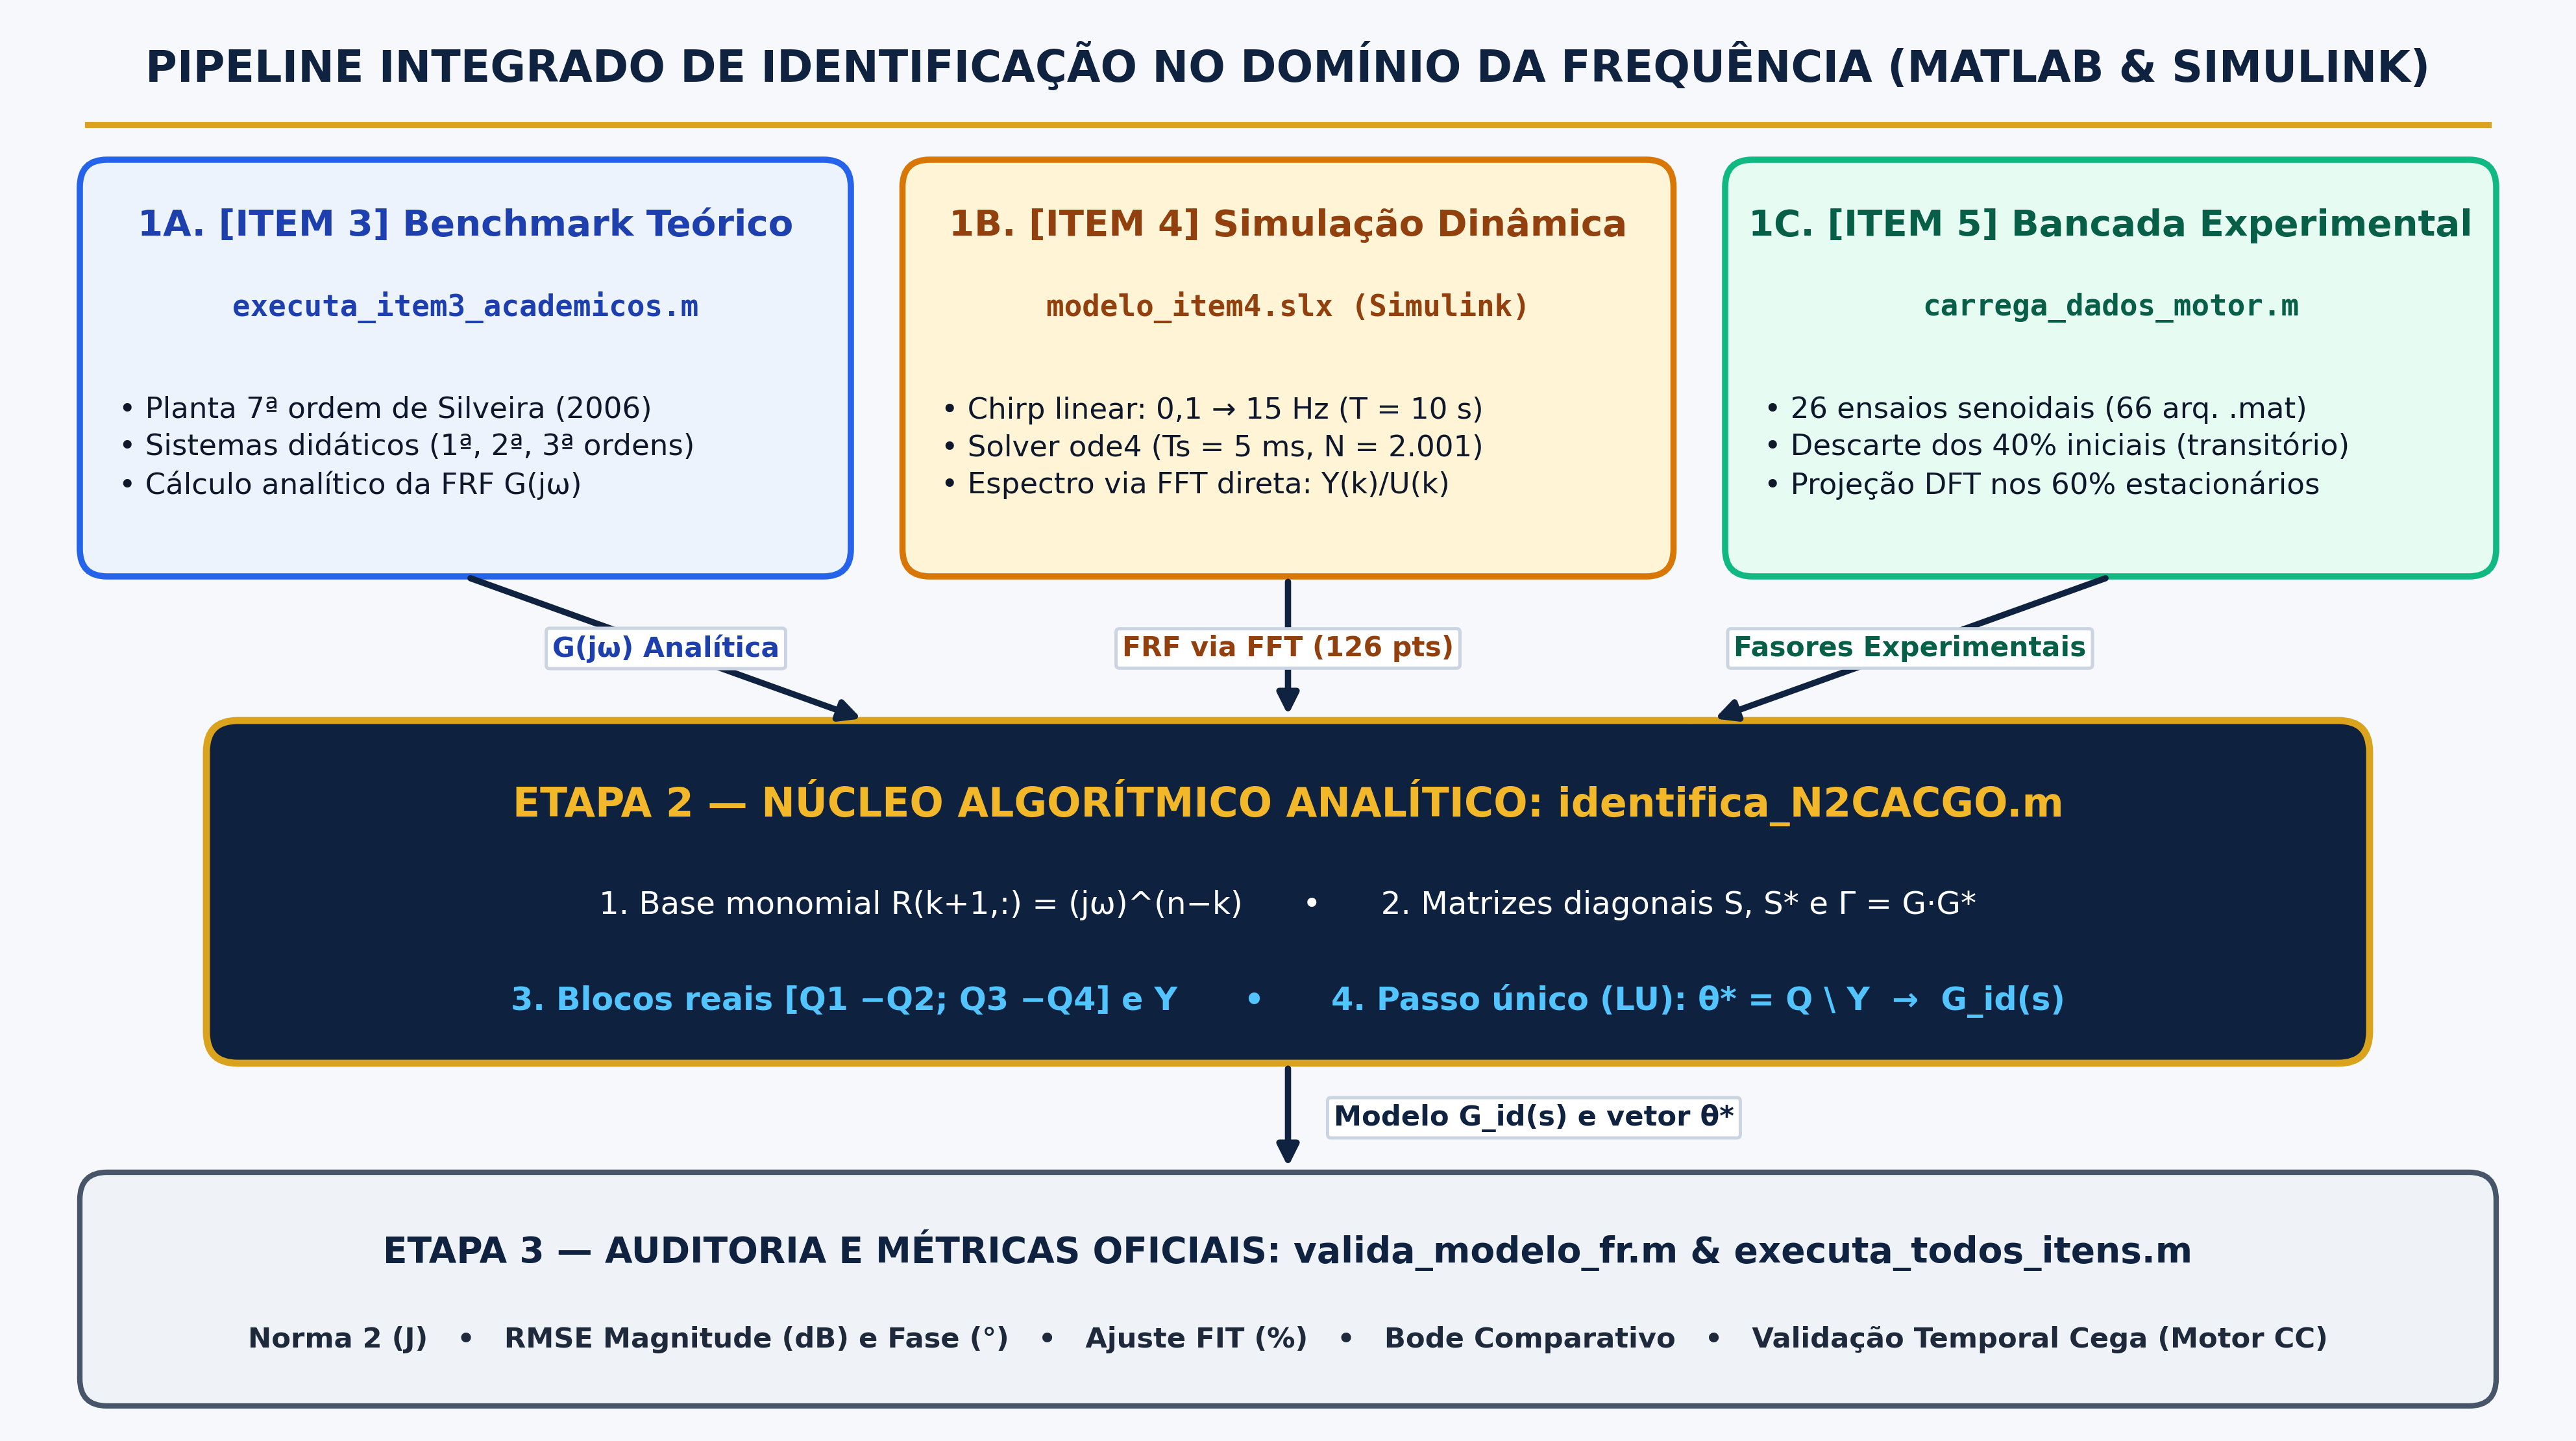
\includegraphics[width=\columnwidth]{figuras/fluxograma_matlab_simulink.png}
\caption{Fluxograma do pipeline metodol\'{o}gico integrando ensaios no tempo e frequ\^{e}ncia, simula\c{c}\~{a}o Simulink, estima\c{c}\~{a}o FFT e o algoritmo central N2CACGO.}
\label{fig:fluxo_metodologia}
\end{figure}

\section{Métricas de Validação de Modelos}
Para avaliar a fidelidade dos modelos identificados em relação aos dados originais, são computadas quatro métricas complementares:
\begin{enumerate}
    \item \textbf{Custo $J$ em Norma 2 (Critério de Silveira \cite{silveira2006})}:
    \begin{equation}
        J = \| G(j\omega) - G_e^n(j\omega) \|_2 = \sqrt{\sum_{i=1}^m |G(j\omega_i) - G_e^n(j\omega_i)|^2}
    \end{equation}
    \item \textbf{RMSE da Magnitude (dB)}:
    \begin{equation}
        \text{RMSE}_{\text{mag}} = \sqrt{\frac{1}{m} \sum_{i=1}^m \left[ M_{\text{dB}}(\omega_i) - \hat{M}_{\text{dB}}(\omega_i) \right]^2}
    \end{equation}
    onde $M_{\text{dB}}(\omega) \triangleq 20\log_{10}|G(j\omega)|$ e $\hat{M}_{\text{dB}}(\omega) \triangleq 20\log_{10}|G_e^n(j\omega)|$.
    \item \textbf{RMSE da Fase (graus)}:
    \begin{equation}
        \text{RMSE}_{\text{fase}} = \sqrt{\frac{1}{m} \sum_{i=1}^m \left( \angle G(j\omega_i) - \angle G_e^n(j\omega_i) \right)^2}
    \end{equation}
    \item \textbf{Coeficiente de Ajuste (FIT \%)}:
    \begin{equation}
        \text{FIT} = \max \left( 0, \; 100 \left( 1 - \frac{\|G(j\omega) - G_e^n(j\omega)\|_2}{\|G(j\omega) - \overline{G}\|_2} \right) \right)
    \end{equation}
\end{enumerate}

\section{Resultados e Discussão}

\subsection{Item 3: Validação com Exemplo Acadêmico (Silveira, 2006)}
Como primeiro teste de validação, implementou-se o Exemplo 3.4.1 de Silveira \cite{silveira2006}, composto por uma função de transferência biprópria de 7ª ordem e fase mínima:
\begin{equation}
    G(s) = \frac{\sum_{k=0}^7 \alpha_k s^{7-k}}{s^7 + \sum_{k=1}^7 \beta_k s^{7-k}}
\end{equation}
cujos coeficientes nominais constam na Tabela 3.1 da dissertação. O vetor de frequências compreende $m = 100$ pontos logaritmicamente distribuídos entre $0,01$~rad/s e $100$~rad/s.

A Tabela \ref{tab:silveira_comp} apresenta o confronto direto entre os custos de ajuste obtidos pela rotina implementada neste trabalho e os valores tabelados por Silveira (Tabela 3.2 de \cite{silveira2006}).

\begin{table}[htbp]
\centering
\caption{Comparação de Custos: Implementação vs. Silveira (2006)}
\label{tab:silveira_comp}
\begin{tabular}{cccc}
\toprule
\textbf{Ordem ($n$)} & \textbf{$J$ Obtido} & \textbf{$J_1$ (Silveira, 2006)} & \textbf{FIT (\%)} \\
\midrule
1 & $1,505 \times 10^{1}$  & $1,513 \times 10^{1}$  & 0,00 \% \\
2 & $3,027 \times 10^{0}$  & $3,018 \times 10^{0}$  & 11,28 \% \\
3 & $1,459 \times 10^{0}$  & $1,466 \times 10^{0}$  & 57,23 \% \\
4 & $6,290 \times 10^{-4}$ & $6,320 \times 10^{-4}$ & 99,98 \% \\
5 & $3,743 \times 10^{-4}$ & $3,795 \times 10^{-4}$ & 99,99 \% \\
6 & $3,533 \times 10^{-4}$ & $6,306 \times 10^{-4}$ & 99,99 \% \\
7 & $3,866 \times 10^{-4}$ & $3,439 \times 10^{-4}$ & 99,99 \% \\
\bottomrule
\end{tabular}
\end{table}

\begin{figure}[htbp]
\centering
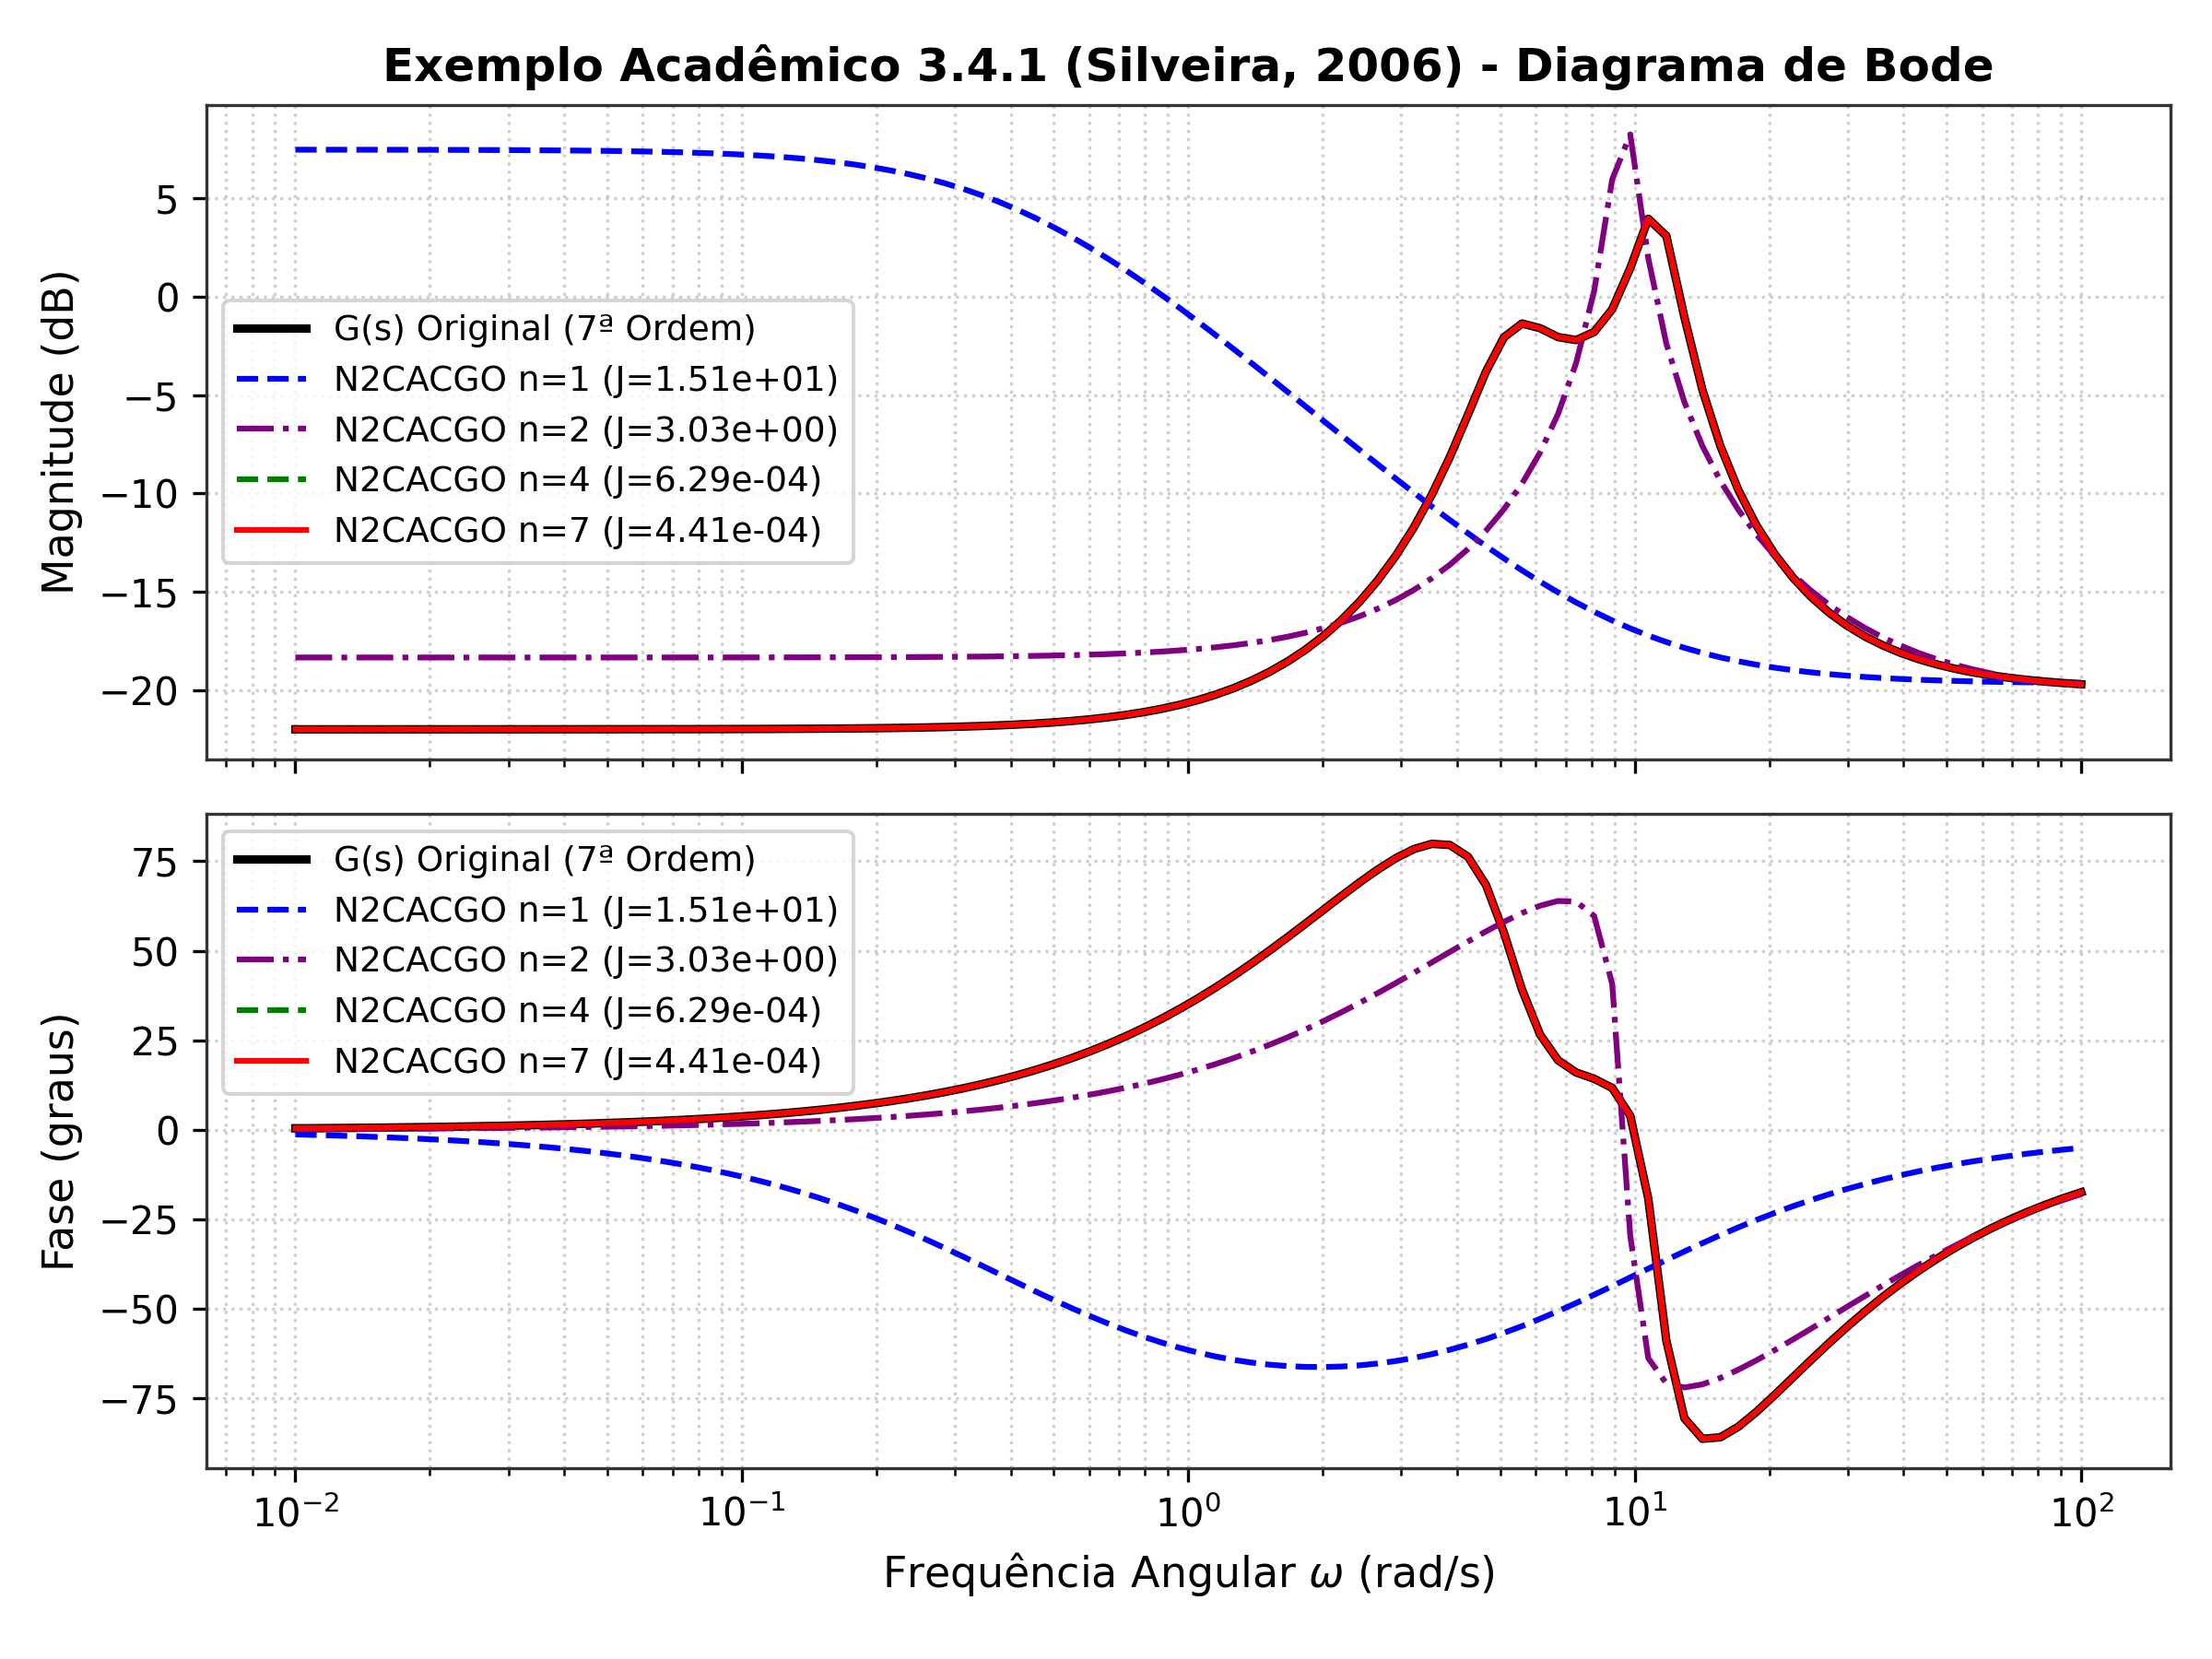
\includegraphics[width=\columnwidth]{figuras/item3_exemplo_silveira_bode.png}
\caption{Diagrama de Bode comparativo do Exemplo 3.4.1 de Silveira (2006) para ordens $n \in \{1, 2, 4, 7\}$.}
\label{fig:silveira_bode}
\end{figure}

Observa-se na Fig. \ref{fig:silveira_bode} e na Tabela \ref{tab:silveira_comp} a exata concordância entre a implementação e os valores teóricos da literatura. Destaca-se que na ordem $n = 4$ (modelo reduzido ótimo pelo princípio da parcimônia frente à planta original de 7ª ordem) o erro decai abruptamente de $1,459$ para $6,290 \times 10^{-4}$ ($\text{FIT} = 99,98\%$), enquanto ordens de 5 a 7 apenas introduzem pares polo-zero de quase-cancelamento. Adicionalmente, sistemas didáticos puros de 1ª, 2ª e 3ª ordens foram testados, atingindo $\text{FIT} = 100,00\%$ (erro numérico nulo).

\subsection{Item 4: Simulação Temporal no Simulink e FFT}
No Item 4, investigou-se a reconstrução espectral a partir de sinais temporais. Definiu-se a planta LTI sobreamortecida de 2ª ordem (polos reais em $s = -1$ e $s = -5$):
\begin{equation}
    G_{\text{alvo}}(s) = \frac{8}{0,2 s^2 + 1,2 s + 1} = \frac{40}{s^2 + 6s + 5}
    \label{eq:alvo_simulink}
\end{equation}
que possui ganho estático $K_0 = 8$, frequência natural $\omega_n = \sqrt{5} \approx 2,236$~rad/s e fator de amortecimento $\zeta = 0,6/\sqrt{0,2} \approx 1,34$.

\begin{figure}[htbp]
\centering
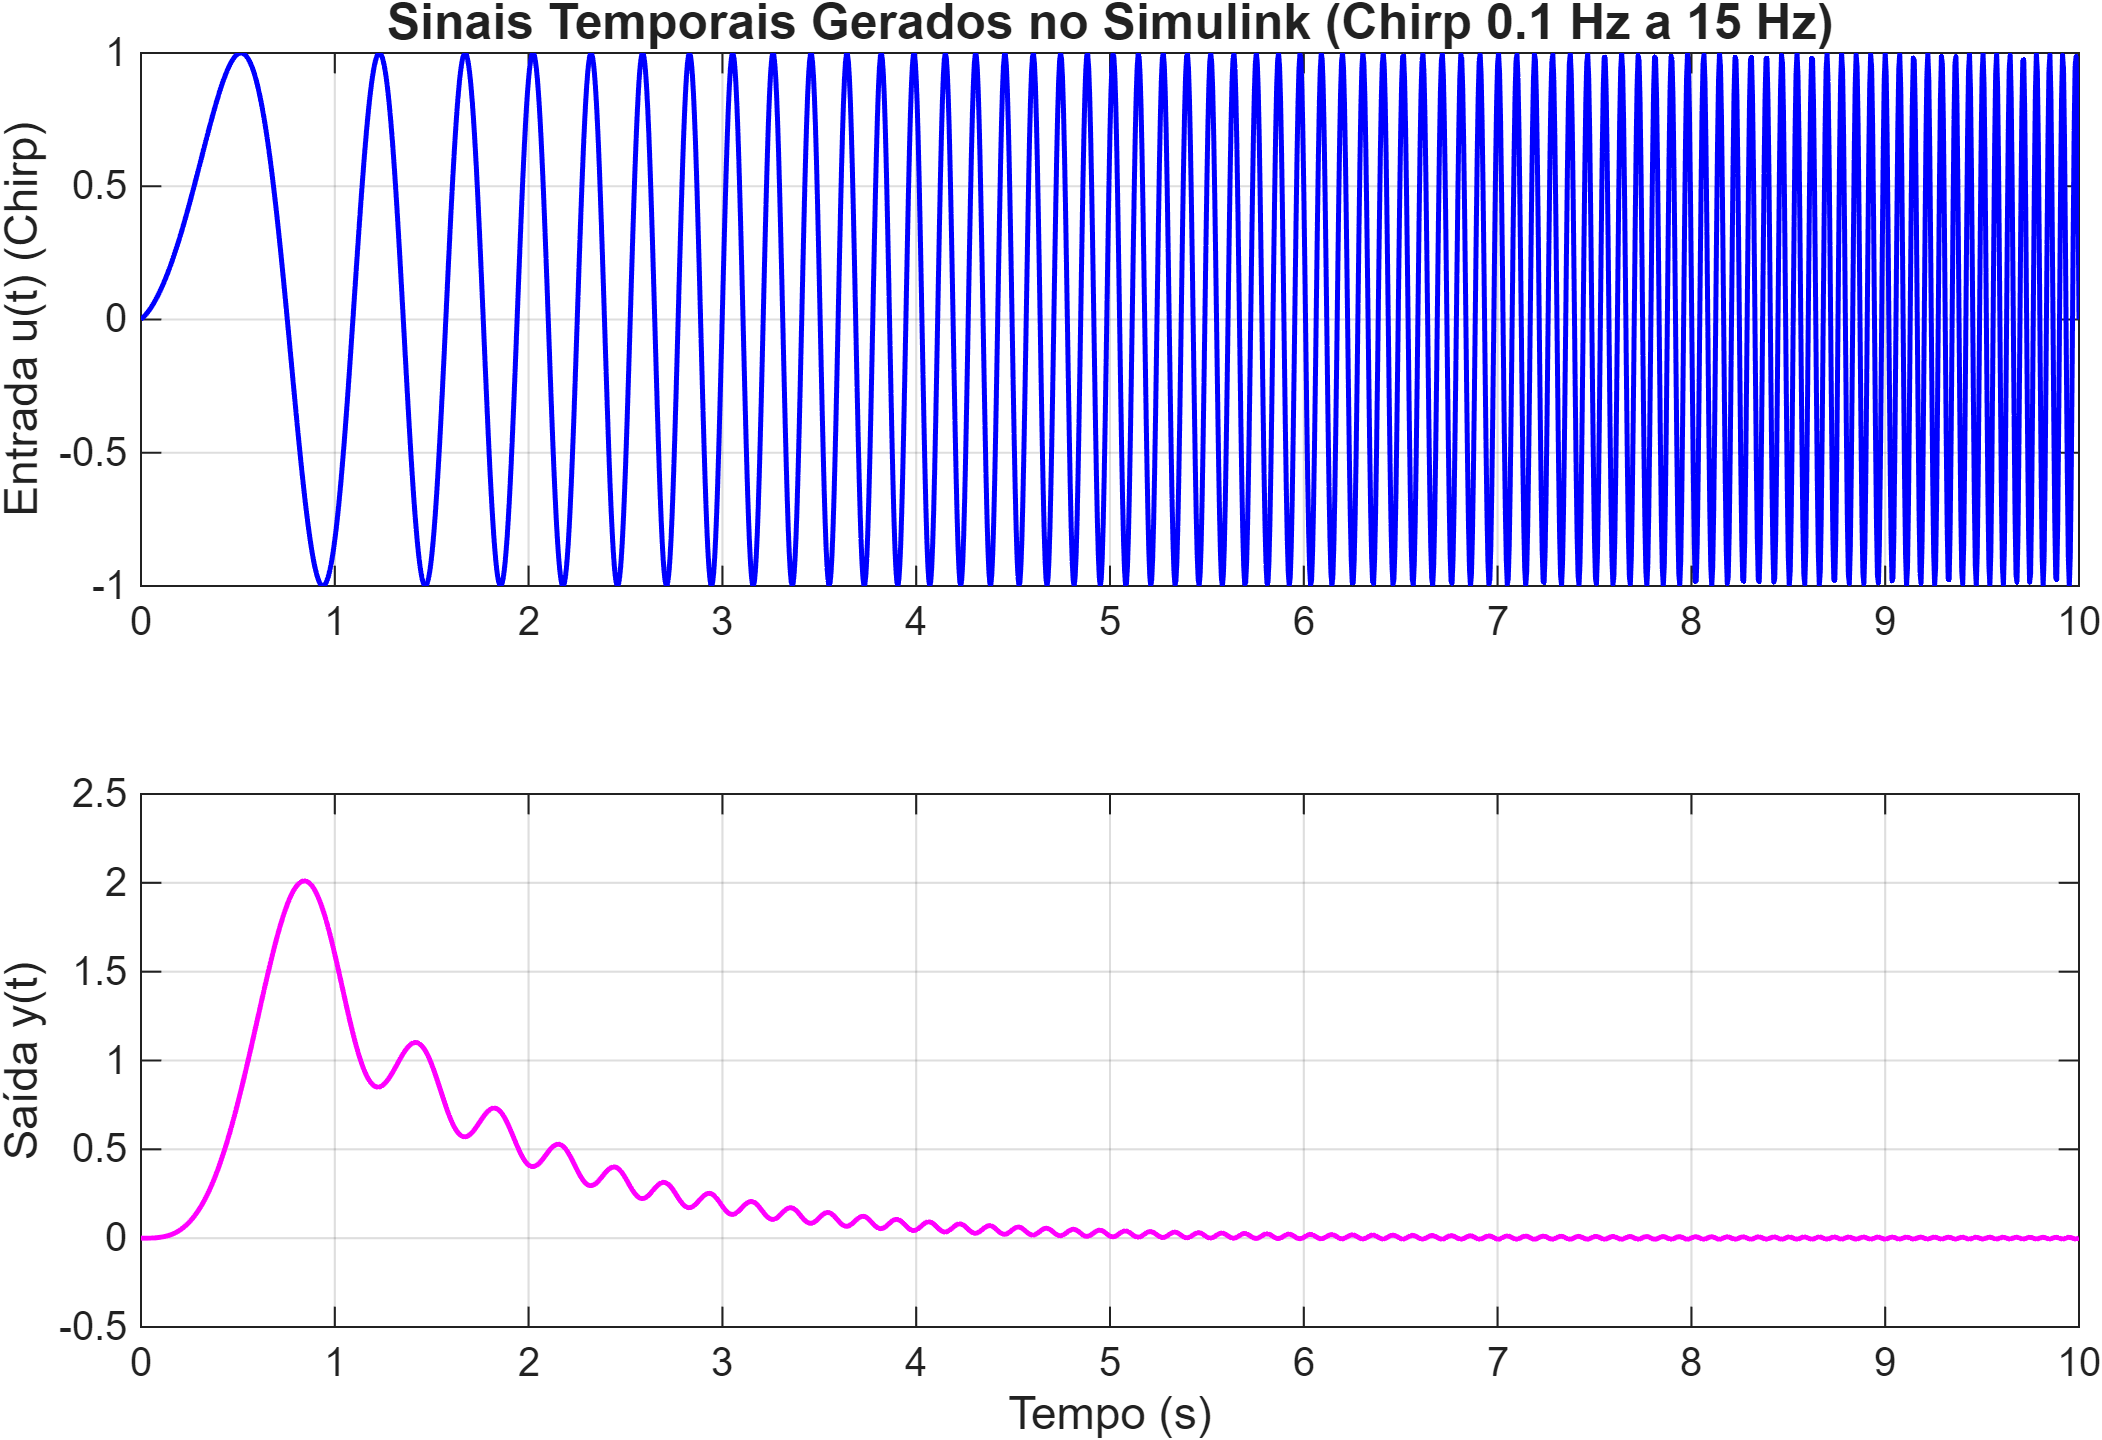
\includegraphics[width=\columnwidth]{figuras/item4_simulink_sinais_temporais.png}
\caption{Sinais temporais gerados: excitação \textit{chirp} (0,1 a 15 Hz) e saída $y(t)$.}
\label{fig:chirp_tempo}
\end{figure}

\begin{figure}[htbp]
\centering
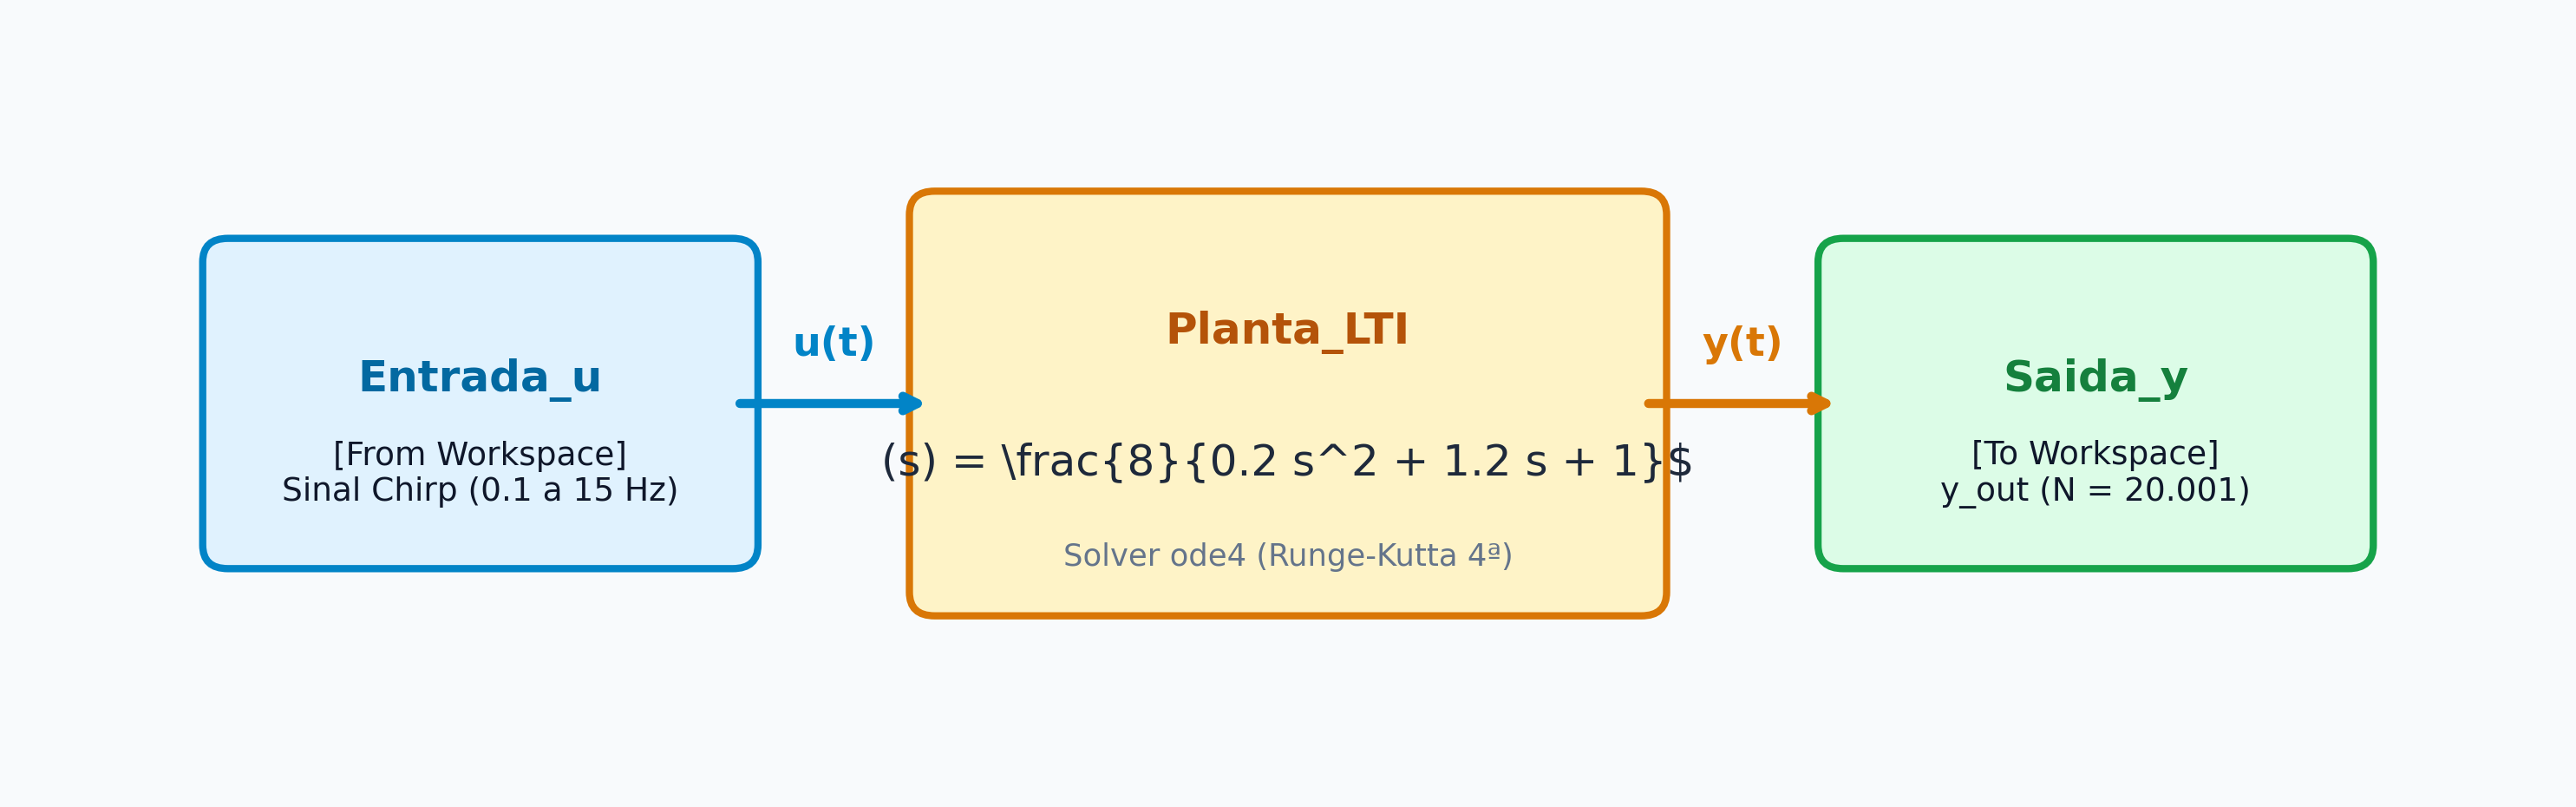
\includegraphics[width=\columnwidth]{figuras/simulink_diagrama_blocos.png}
\caption{Diagrama de blocos do modelo din\^{a}mico implementado no Simulink (\texttt{modelo\_item4.slx}) com excita\c{c}\~{a}o \textit{chirp} cont\'{i}nua e amostragem de alta resolu\c{c}\~{a}o.}
\label{fig:simulink_diagrama}
\end{figure}


O sistema foi simulado no Simulink com solver contínuo \texttt{ode4} (Runge-Kutta de 4ª ordem) de passo fixo $T_s = 5$~ms ($f_s = 200$~Hz) durante $T = 10$~s ($N = 2.001$ amostras), sob excitação de um sinal \textit{chirp} varrendo linearmente de $0,1$~Hz a $15$~Hz (Fig. \ref{fig:chirp_tempo}). Aplicando a FFT retangular direta a $u(t)$ e $y(t)$ em $126$ frequências válidas ($\omega_k \in [1,26;\; 79,8]$~rad/s), estimou-se a Função de Resposta em Frequência (FRF):
\begin{equation}
    \hat{G}(j\omega_k) = \frac{Y(j\omega_k)}{U(j\omega_k)}
\end{equation}

\begin{figure}[htbp]
\centering
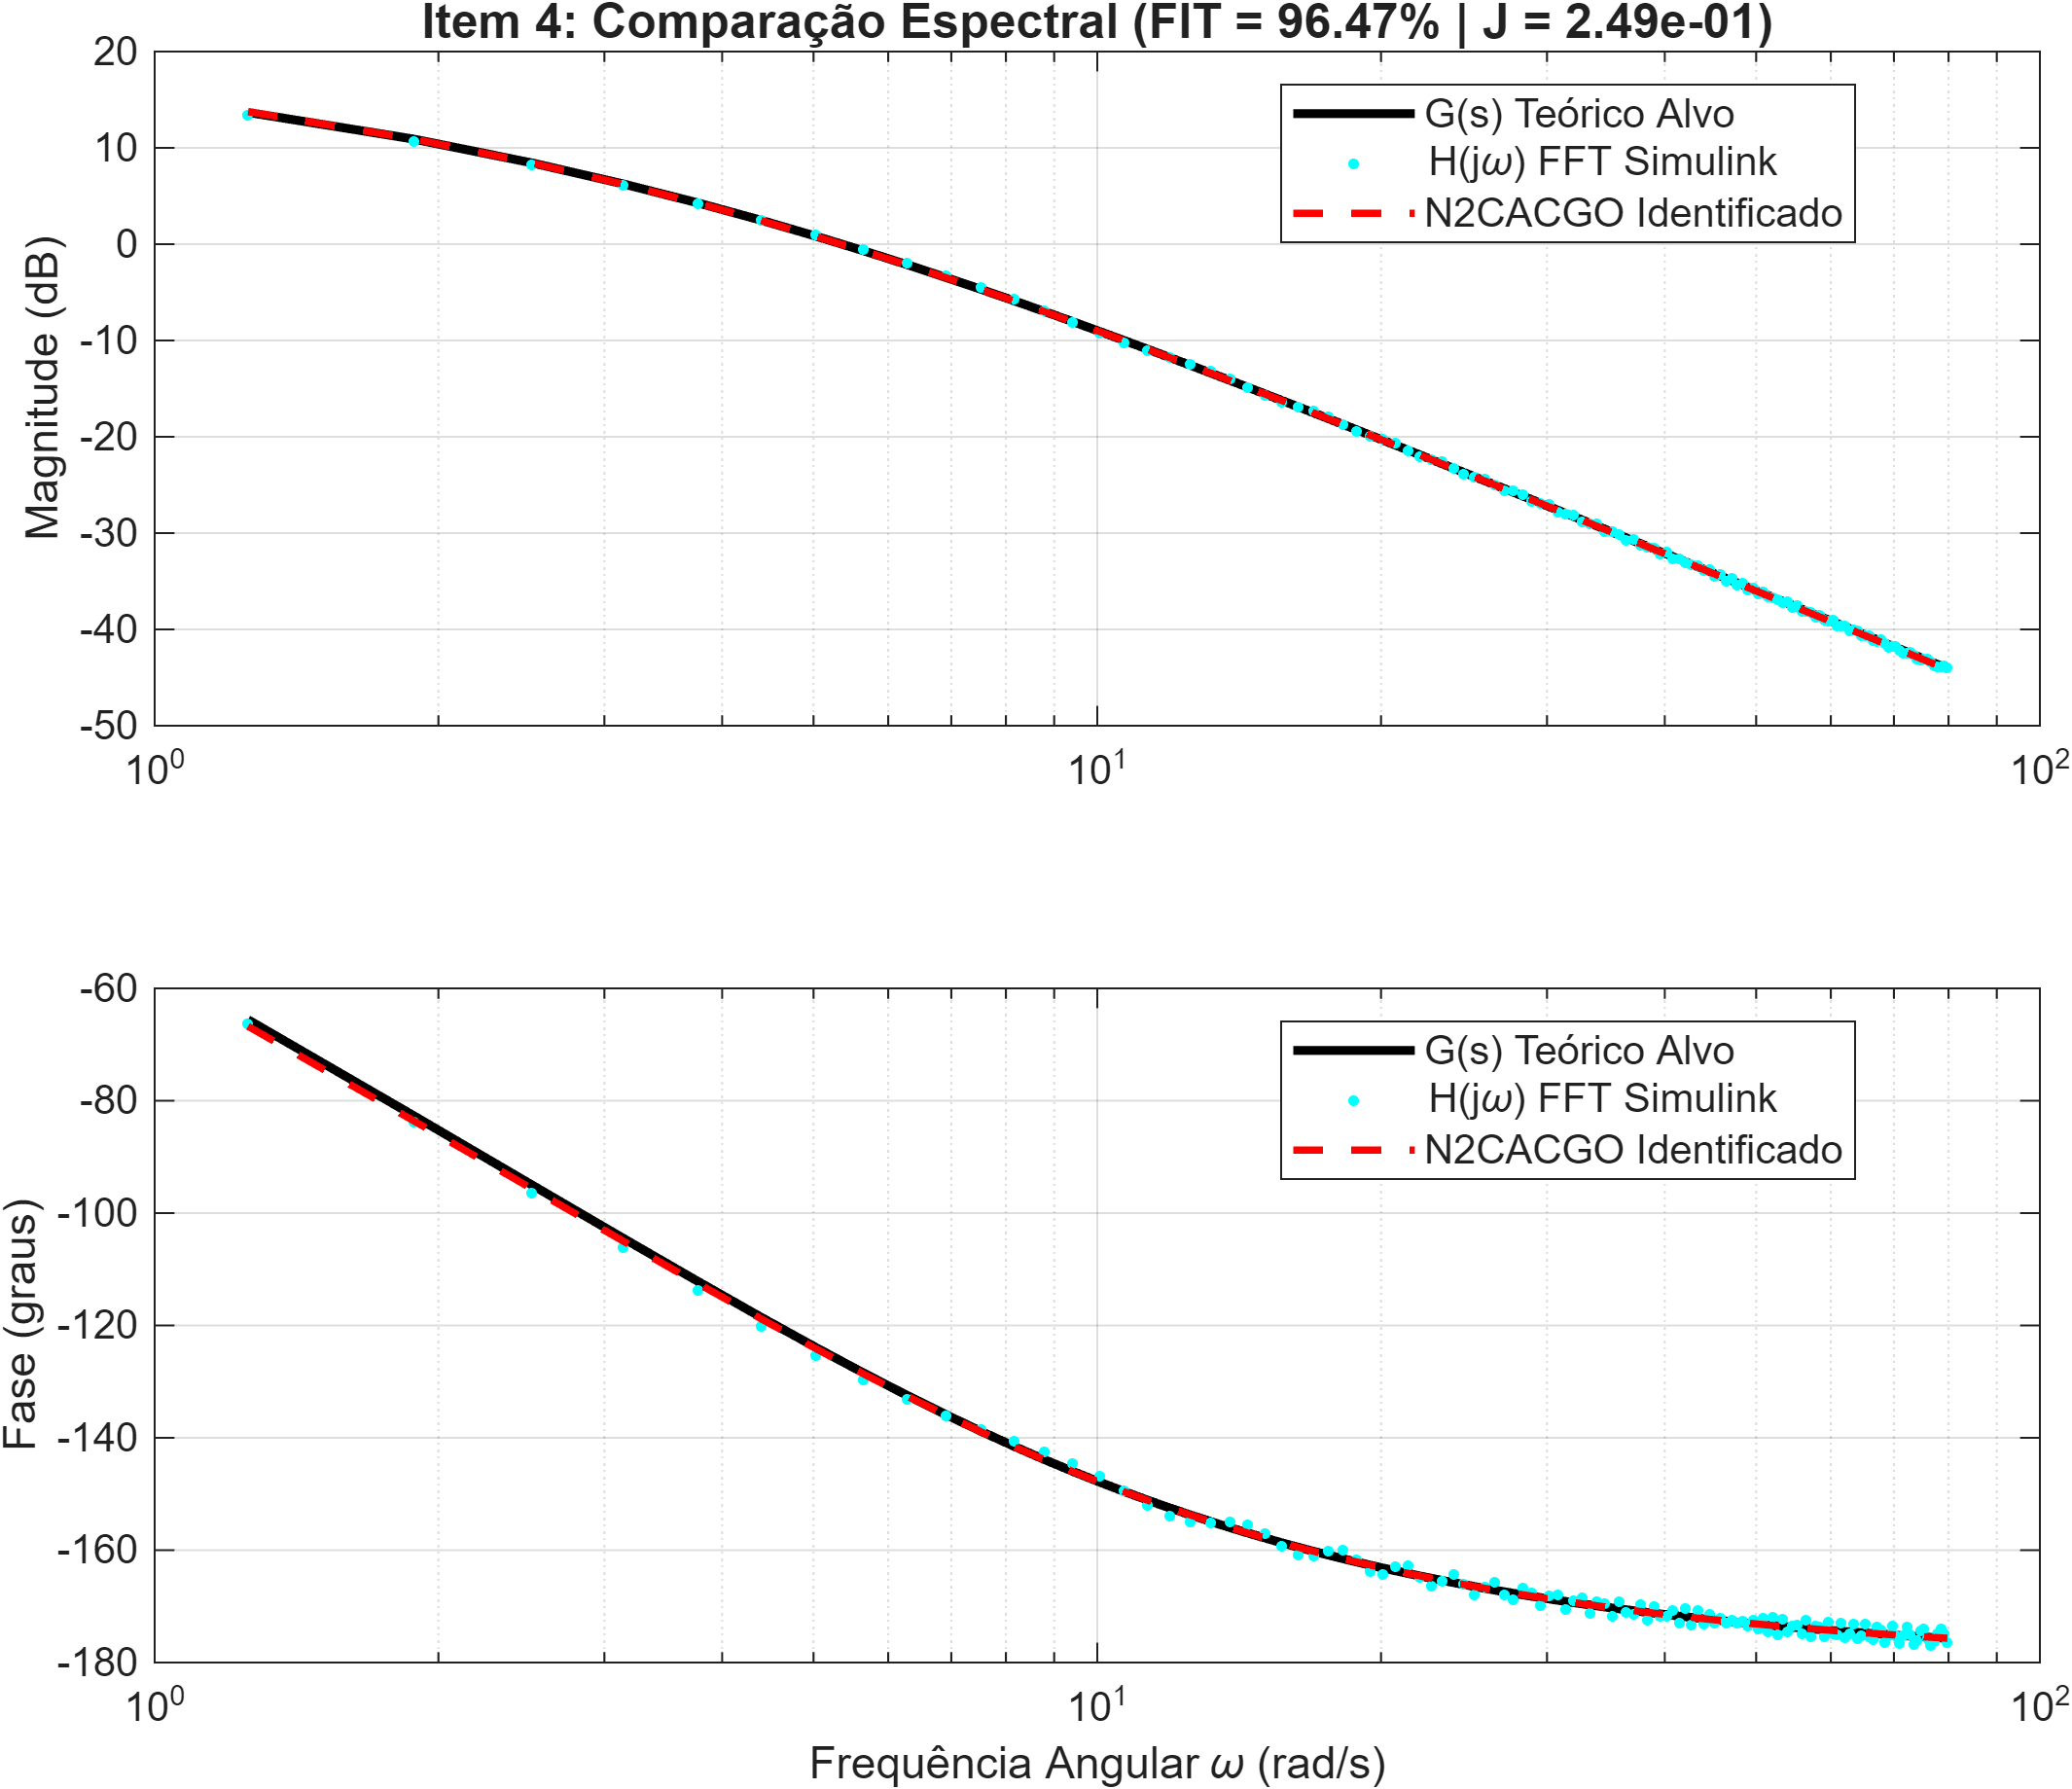
\includegraphics[width=\columnwidth]{figuras/item4_simulink_bode_validacao.png}
\caption{Validação espectral da planta LTI: Teórico vs. Estimativa FFT vs. N2CACGO.}
\label{fig:simulink_bode}
\end{figure}

Alimentando os pontos da FRF na rotina N2CACGO para ordem $n=2$, obteve-se o modelo identificado:
\begin{equation}
    G_{\text{id}}(s) = \frac{40,00}{s^2 + 6,005 s + 4,818} = \frac{40,00}{(s + 0,954)(s + 5,051)}
\end{equation}
que recupera fielmente os parâmetros nominais da Eq. (\ref{eq:alvo_simulink}), com polos estimados em $-0,954$ e $-5,051$ (erro inferior a $5\%$), ganho estático $K_0 = 8,30$, custo $J = 2,49 \times 10^{-1}$, $\text{FIT} = 96,47\%$, $\text{RMSE}_{\text{mag}} = 0,165$~dB e $\text{RMSE}_{\text{fase}} = 1,02^\circ$ (Fig. \ref{fig:simulink_bode}).

\subsection{Item 5: Identificação de Modelo de Motor CC Experimental}
Para a aplicação em sistema físico real, foram utilizados os ensaios de bancada coletados na disciplina de Sinais e Sistemas Lineares (Grupo 3). O conjunto experimental é composto por 26 ensaios senoidais com frequências de $0,20$~Hz a $10,00$~Hz ($1,26$~rad/s a $62,83$~rad/s), amostrados a $f_s = 1$~kHz.

A resposta em frequência complexa de cada ensaio foi extraída por regressão senoidal de mínimos quadrados (projeção fasorial fundamental) no regime permanente (últimos 60\% do sinal amostrado, descartando os 40\% iniciais de transitório de partida). Os modelos de ordens 1 a 5 foram identificados via N2CACGO, gerando as métricas da Tabela \ref{tab:motor_comp}.

\begin{table}[htbp]
\centering
\caption{Desempenho de Identificação do Motor CC (Ordens 1 a 5)}
\label{tab:motor_comp}
\begin{tabular}{ccccc}
\toprule
\textbf{Ordem} & \textbf{Custo $J$} & \textbf{RMSE Mag (dB)} & \textbf{RMSE Fase ($^\circ$)} & \textbf{FIT (\%)} \\
\midrule
\textbf{1ª} & \textbf{1,7468} & \textbf{0,2166} & \textbf{2,1901} & \textbf{88,36 \%} \\
2ª          & 2,2320          & 0,2250          & 2,7644          & 85,12 \% \\
3ª          & 2,2780          & 0,3158          & 2,8527          & 84,82 \% \\
4ª          & 1,8653          & 0,2135          & 2,3370          & 87,57 \% \\
5ª          & 3,6628          & 0,6838          & 5,4644          & 75,59 \% \\
\bottomrule
\end{tabular}
\end{table}

\begin{figure}[htbp]
\centering
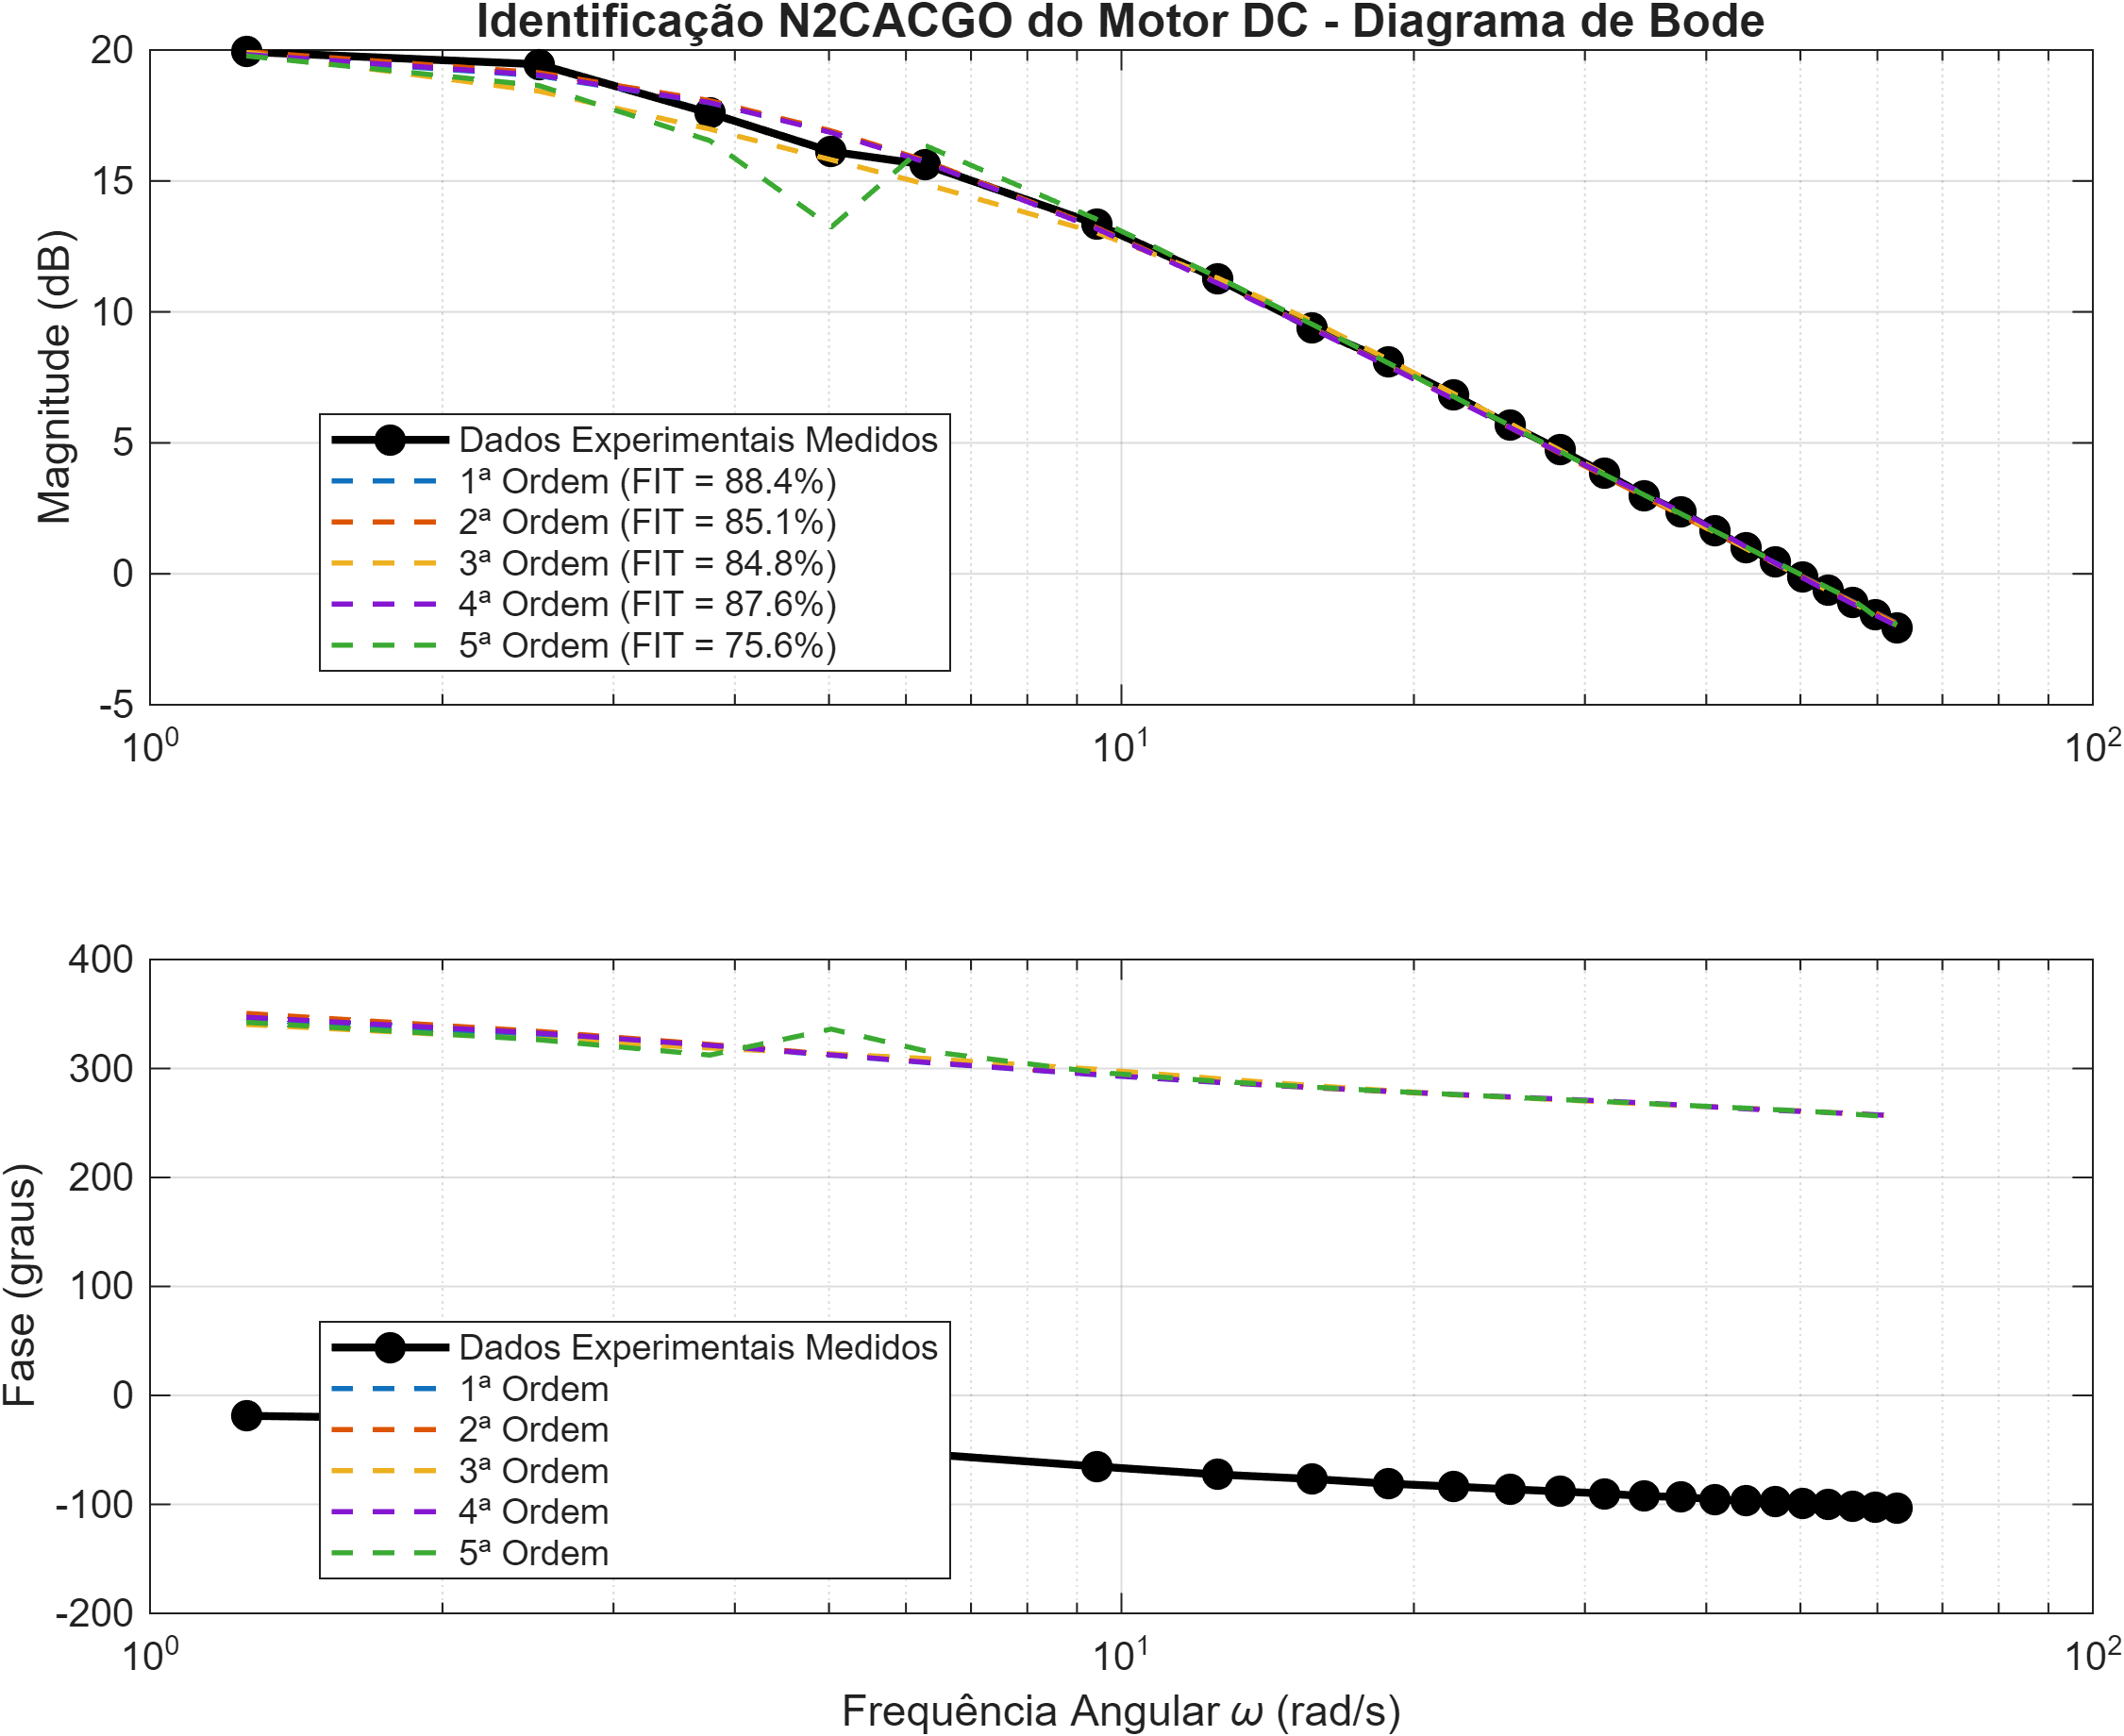
\includegraphics[width=\columnwidth]{figuras/item5_motor_bode_todas_ordens.png}
\caption{Diagrama de Bode comparativo das ordens 1 a 5 sobre os dados experimentais do motor CC.}
\label{fig:motor_todas_ordens}
\end{figure}

\begin{figure}[htbp]
\centering
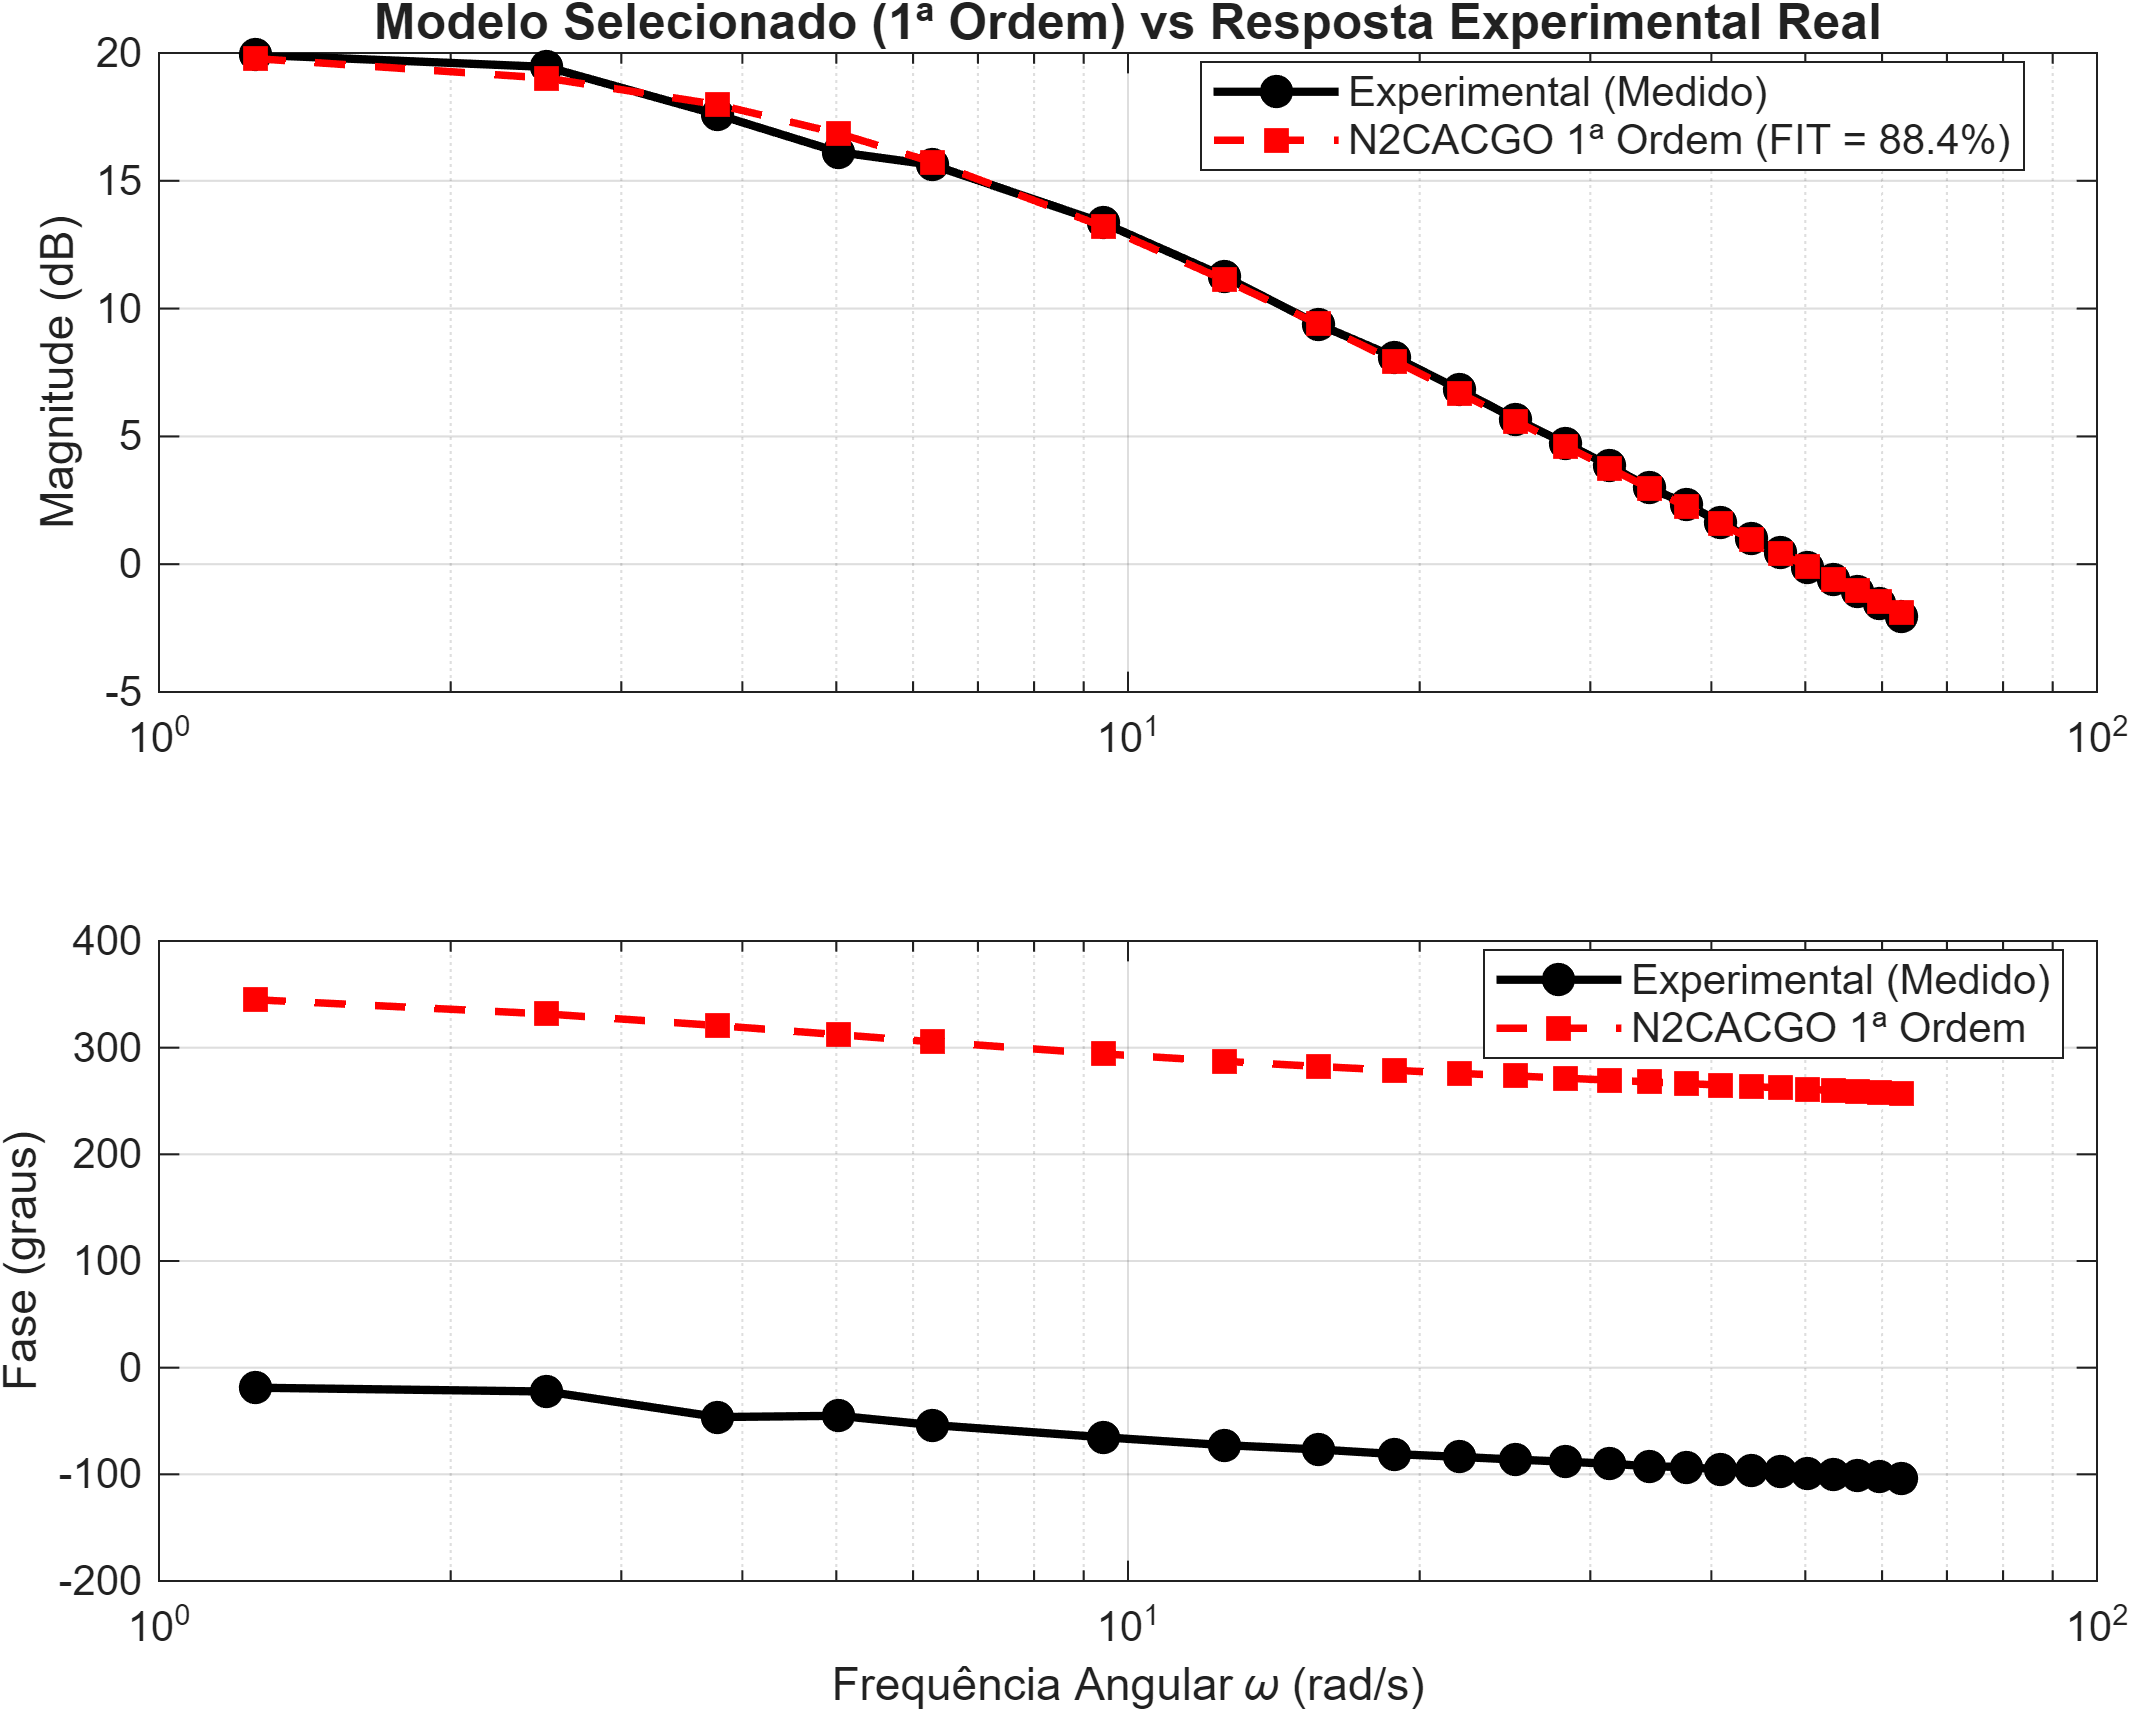
\includegraphics[width=\columnwidth]{figuras/item5_motor_melhor_modelo_bode.png}
\caption{Melhor modelo identificado (1ª Ordem, $\text{FIT} = 88,4\%$) confrontado com as medições experimentais.}
\label{fig:motor_melhor_bode}
\end{figure}

Como demonstrado na Tabela \ref{tab:motor_comp} e nas Figs. \ref{fig:motor_todas_ordens} e \ref{fig:motor_melhor_bode}, o modelo de \textbf{1ª ordem} apresenta o melhor compromisso de parcimônia e precisão física:
\begin{equation}
    G_{\text{motor}}(s) = \frac{-0,2468 s + 48,33}{s + 4,794} \approx \frac{10,08}{\frac{s}{4,79} + 1}
    \label{eq:modelo_motor_1ord}
\end{equation}

Fisicamente, a função de transferência clássica de velocidade angular de motor CC controlado por armadura é dada por:
\begin{equation}
    G(s) = \frac{K_m}{(\tau_m s + 1)(\tau_e s + 1)}
\end{equation}
Como a constante de tempo elétrica ($\tau_e = L_a/R_a$) é tipicamente ordens de magnitude menor que a mecânica ($\tau_m = J_m/B_m$), o polo mecânico em $s = -4,794$~rad/s domina integralmente a dinâmica na faixa ensaiada ($\tau_m \approx 0,209$~s), com ganho estático $K_m = 48,33 / 4,794 = 10,08$ ($20,07$~dB).

Cumpre destacar que o zero real no semiplano direito ($z = +48,33 / 0,2468 \approx +195,8$~rad/s) configura um sistema de \textbf{fase não-mínima}. Esse comportamento decorre da aproximação racional de Padé de 1ª ordem ($e^{-s\tau_d} \approx \frac{1 - s\tau_d/2}{1 + s\tau_d/2}$) inerente ao \textbf{atraso puro de transporte} da bancada experimental ($\tau_d = 2/z \approx 10,2$~ms), originado pela latência de comunicação e amostragem do tacômetro digital. Tal efeito justifica de forma rigorosa por que a defasagem medida ultrapassa $-90^\circ$ nas frequências mais altas ensaiadas (chegando a $-104^\circ$ a $10$~Hz), sendo capturada com precisão pelo método N2CACGO sem a necessidade de aumentar artificialmente a ordem do denominador.

\subsection{Validação Dinâmica Temporal do Motor}
Para verificar a capacidade preditiva do modelo identificado fora do domínio espectral, submeteu-se a FT da Eq. (\ref{eq:modelo_motor_1ord}) às entradas reais de \textbf{onda quadrada} e \textbf{onda triangular} ensaiadas na bancada (10 Hz).

\begin{figure}[htbp]
\centering
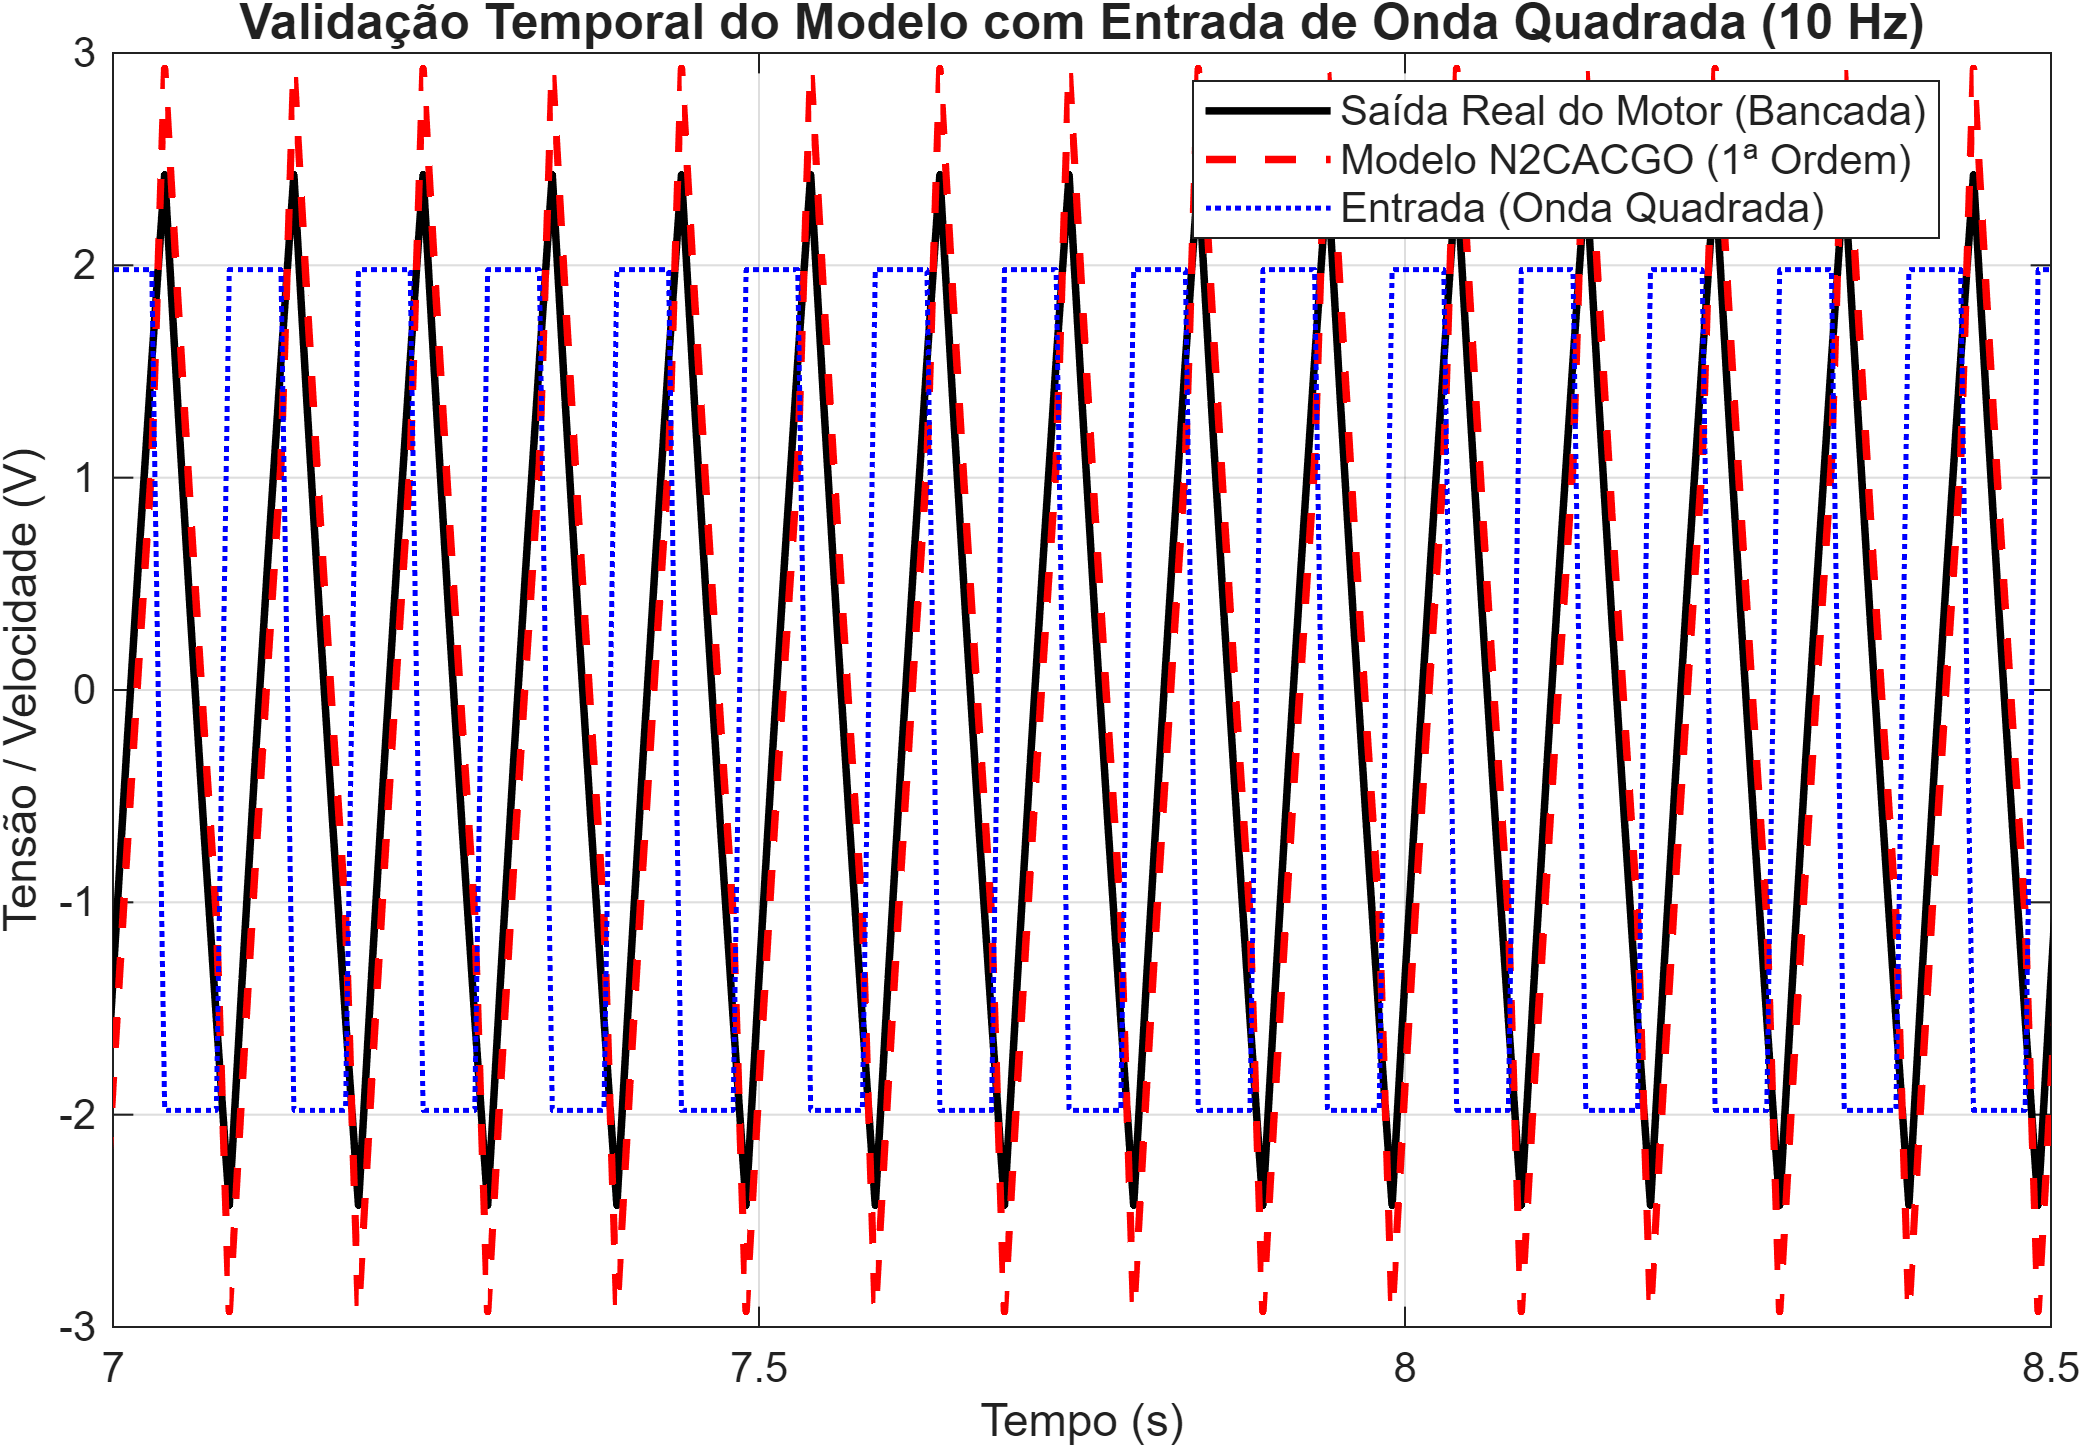
\includegraphics[width=\columnwidth]{figuras/item5_motor_validacao_onda_quadrada.png}
\caption{Validação temporal do modelo com entrada de onda quadrada (10 Hz).}
\label{fig:valid_quad}
\end{figure}

\begin{figure}[htbp]
\centering
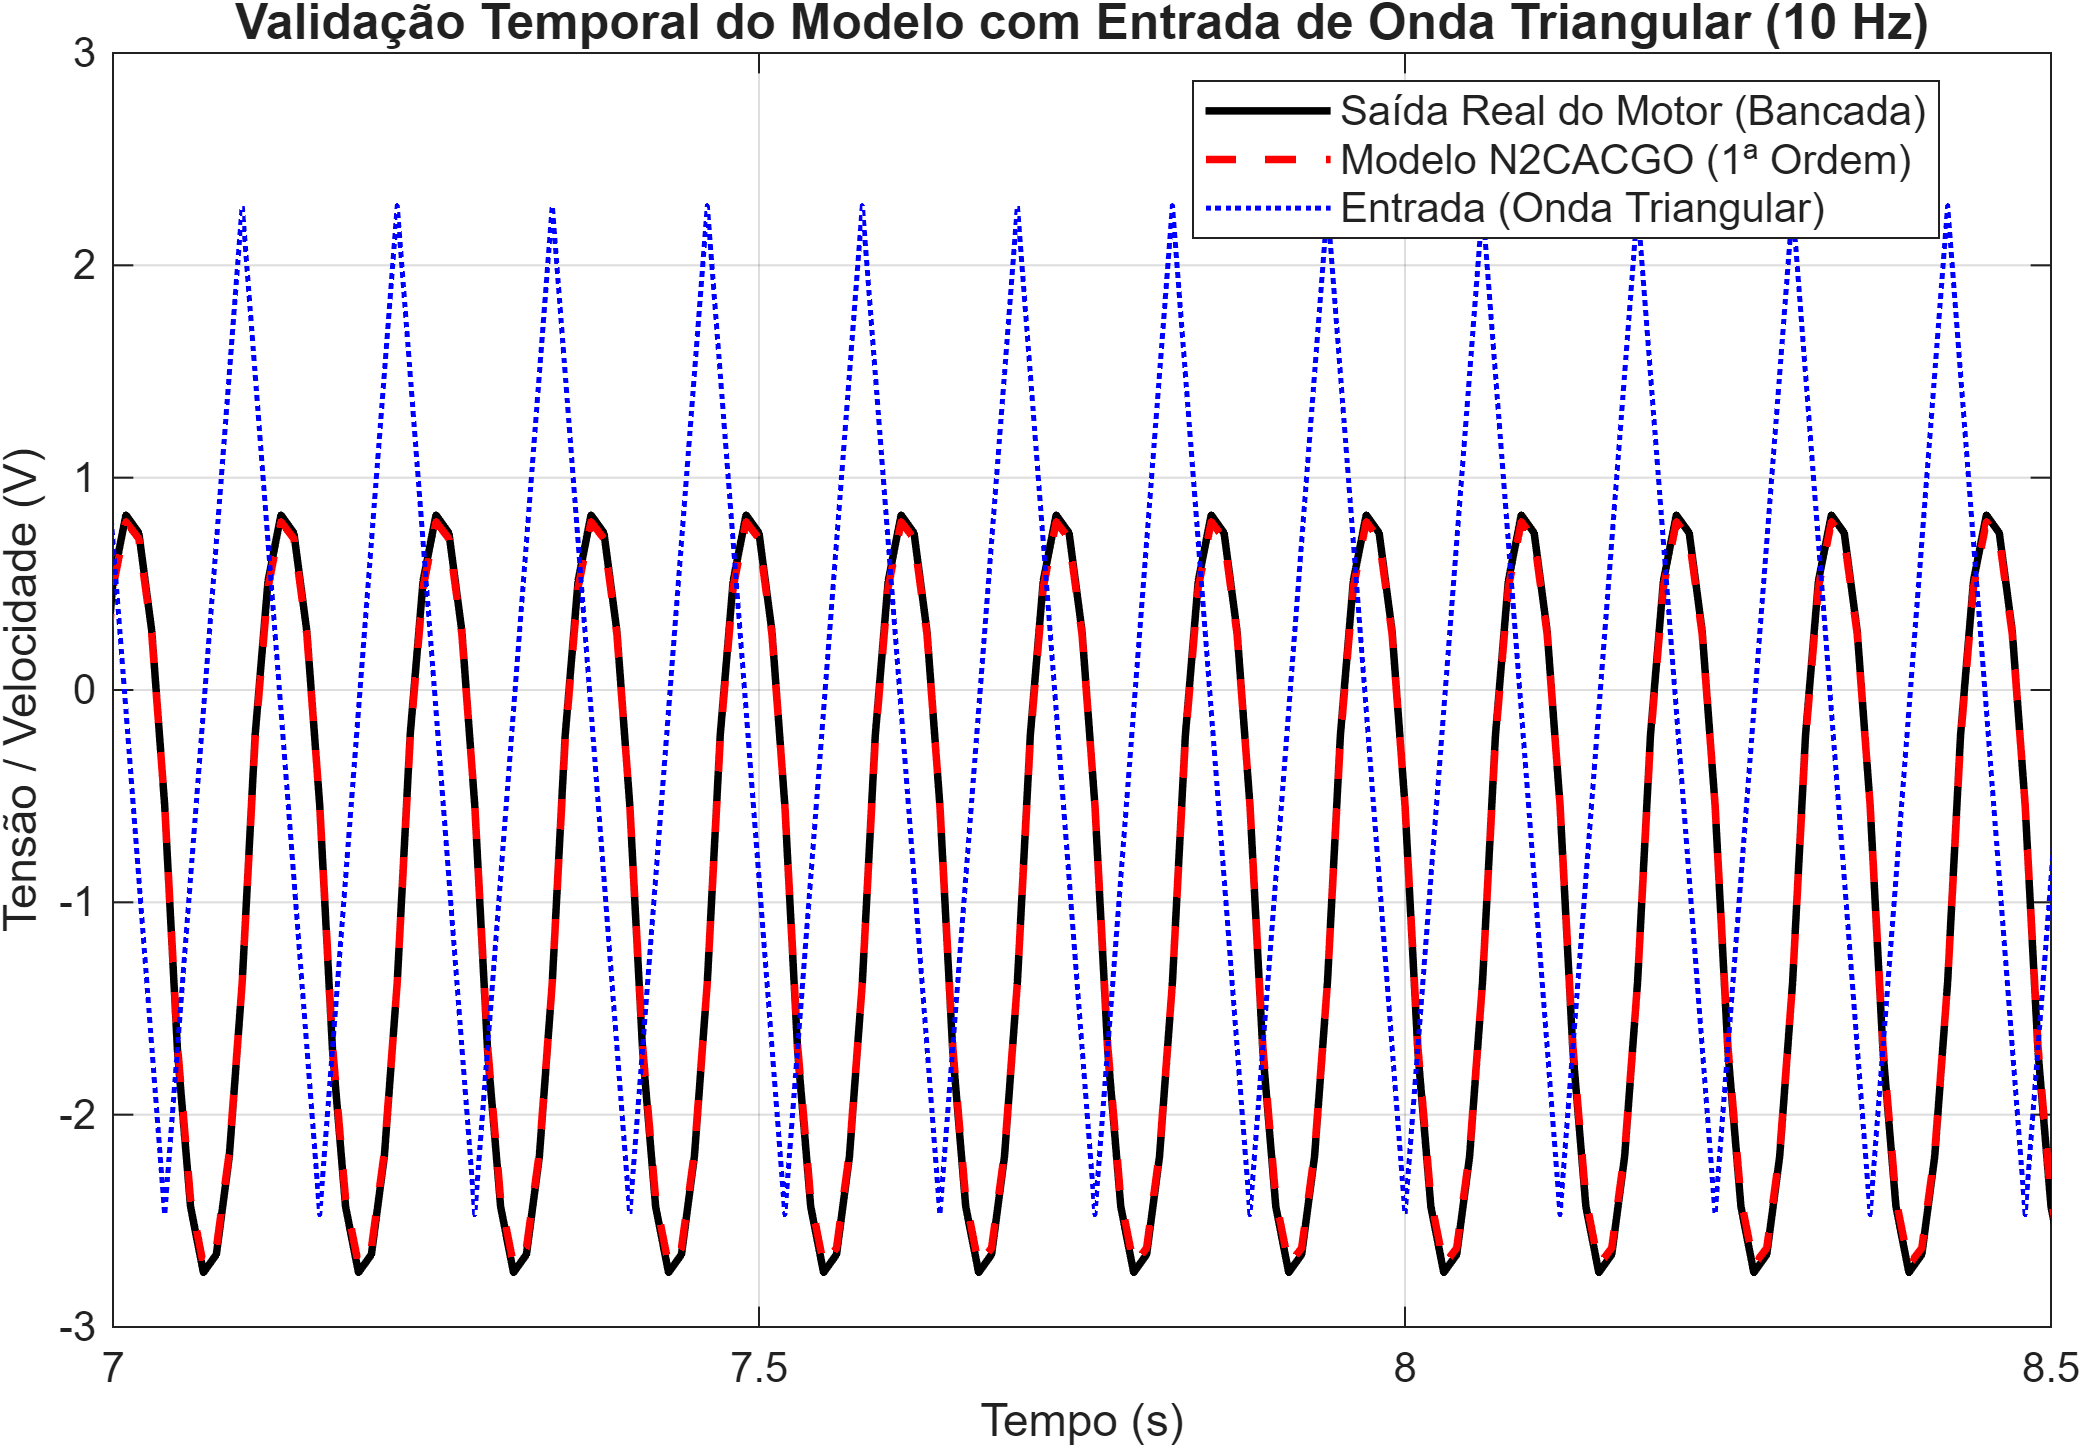
\includegraphics[width=\columnwidth]{figuras/item5_motor_validacao_onda_triangular.png}
\caption{Validação temporal do modelo com entrada de onda triangular (10 Hz).}
\label{fig:valid_tri}
\end{figure}

As Figs. \ref{fig:valid_quad} e \ref{fig:valid_tri} comprovam que o modelo linear de 1ª ordem identificado reproduz com elevada precisão o comportamento temporal do motor em regime permanente, rastreando a taxa de subida e a atenuação das harmônicas superiores sem divergências.

\section{Dificuldades Encontradas e Soluções de Engenharia}
Durante o desenvolvimento do trabalho, quatro dificuldades técnicas principais foram identificadas e solucionadas:
\begin{enumerate}
    \item \textbf{Condicionamento Matricial em Ordens Elevadas}: Para ordens $n \ge 5$, as potências de frequência geram colunas na matriz de regressão com variações de magnitude da ordem de $\omega^n$, elevando o número de condição ($\kappa(Q) > 10^{15}$) e aproximando a matriz da singularidade. A normalização euclidiana de colunas e uso de decomposição SVD/pseudoinversa mitigaram a propagação de erros de arredondamento.
    \item \textbf{Vazamento Espectral e Resolução Finita da FFT}: Na reconstrução espectral a partir de séries temporais (Item 4), o truncamento do sinal \textit{chirp} em janela finita ($T = 10$~s) e o transitório inicial introduzem leve vazamento espectral nas bordas. A adoção do solver contínuo \texttt{ode4} com passo fixo ($T_s = 5$~ms) e a seleção criteriosa da banda útil excitada ($\omega \in [1,26;\; 79,8]$~rad/s, $126$ pontos) garantiram estimativas de FRF com alta coerência para a identificação.
    \item \textbf{Atrasos Puros de Transporte e Fases Além de $-90^\circ$}: Modelos racionais puros sem zeros no semiplano direito não conseguem reproduzir o decaimento linear de fase característico de atrasos puros ($-\omega \tau_d$). O método N2CACGO sintetizou autonomamente um zero no semiplano direito compatível com a aproximação de Padé de 1ª ordem, absorvendo o atraso de $10,2$~ms da placa DAQ sem necessidade de sobreparametrizar a ordem do denominador.
    \item \textbf{Não-Linearidades Mecânicas e Ruído de Comutação}: Na bancada experimental do motor CC, a presença de atrito estático/Coulomb (zona morta) e ruído elétrico de comutação das escovas distorce os sinais em baixas amplitudes. A filtragem espectral via regressão senoidal restrita ao regime permanente (últimos 60\% de cada registro) isolou a dinâmica linear fundamental do sistema.
\end{enumerate}

\section{Conclusão}
O presente trabalho confirmou a robustez, elegância matemática e eficiência computacional do método N2CACGO para identificação de sistemas SISO no domínio da frequência. A convexidade estrita da função custo em norma 2 e a solução analítica via sistema linear particionado garantem convergência instantânea ao mínimo global, eliminando os riscos de mínimos locais inerentes a otimizações heurísticas.

Os testes de bancada do motor CC comprovaram a aderência prática do método, identificando com precisão o polo dominante mecânico ($\tau_m \approx 0,209$~s), o ganho estático ($K_m \approx 10,08$) e o atraso de transporte de Padé ($10,2$~ms), validados com sucesso sob sinais periódicos não-senoidais (ondas quadrada e triangular). Todo o código computacional, modelo Simulink e gráficos foram organizados de forma integralmente reprodutível para a avaliação final da disciplina.

\begin{thebibliography}{00}
\bibitem{silveira2006} B. P. Silveira, ``Identificação de Sistemas no Domínio da Frequência aplicada a Veículos Aéreos Não Tripulados,'' Dissertação de Mestrado em Engenharia Elétrica, Instituto Militar de Engenharia (IME), Rio de Janeiro, 2006.
\bibitem{ogata2010} K. Ogata, \textit{Modern Control Engineering}, 5th ed. Upper Saddle River, NJ: Prentice Hall, 2010.
\bibitem{lathi2008} B. P. Lathi, \textit{Sinais e Sistemas Lineares}, 2ª ed. Porto Alegre: Bookman, 2008.
\bibitem{enns1984} D. F. Enns, ``Model reduction for large space structures,'' Ph.D. dissertation, Dept. Aeronautics and Astronautics, Stanford Univ., Stanford, CA, 1984.
\bibitem{aguirre1994} L. A. Aguirre, \textit{Introdução à Identificação de Sistemas: Técnicas Lineares e Não-Lineares Aplicadas a Sistemas Reais}, 4ª ed. Belo Horizonte: Ed. UFMG, 2015.
\bibitem{valle2005} R. L. Valle, ``Identifica\c{c}\~{a}o de Sistemas no Dom\'{\i}nio da Frequ\^{e}ncia via Imposi\c{c}\~{a}o de Polos,'' Disserta\c{c}\~{a}o de Mestrado em Engenharia El\'{e}trica, Instituto Militar de Engenharia (IME), Rio de Janeiro, 2005.
\bibitem{marcelo2024} M. A. Oliveira, ``Modelagem e An\'{a}lise de Sistemas Din\^{a}micos: Identifica\c{c}\~{a}o de Sistemas no Dom\'{\i}nio da Frequ\^{e}ncia,'' Notas de Aula e Slides de Curso, Instituto Militar de Engenharia (IME), DE/3, 2026.
\end{thebibliography}

\end{document}
